\documentclass[11pt,a4paper]{article}

% === Packages ===
\usepackage[utf8]{inputenc}
\usepackage[T1]{fontenc}
\usepackage{amsmath,amssymb,amsthm}
\usepackage{enumitem}
\usepackage{hyperref}
\usepackage{cleveref}
\usepackage{tikz}
\usepackage{tikz-cd}
\usetikzlibrary{positioning,arrows.meta,calc,patterns,decorations.pathreplacing}
\usepackage{booktabs}
\usepackage{geometry}
\usepackage{xcolor}
\usepackage{tcolorbox}
\usepackage{longtable}
\usepackage{array}
\usepackage{mathtools}

\geometry{margin=1in}
\hypersetup{colorlinks=true,linkcolor=blue!70!black,citecolor=green!50!black,urlcolor=purple!70!black}

% === Theorem environments ===
\theoremstyle{plain}
\newtheorem{theorem}{Theorem}[section]
\newtheorem{proposition}[theorem]{Proposition}
\newtheorem{lemma}[theorem]{Lemma}
\newtheorem{corollary}[theorem]{Corollary}
\newtheorem{conjecture}[theorem]{Conjecture}

\theoremstyle{definition}
\newtheorem{definition}[theorem]{Definition}
\newtheorem{example}[theorem]{Example}
\newtheorem{remark}[theorem]{Remark}
\newtheorem{audit}[theorem]{CRM Audit}
\newtheorem{prediction}[theorem]{Prediction}
\newtheorem{observation}[theorem]{Observation}

% === Macros ===
\newcommand{\BISH}{\textsf{BISH}}
\newcommand{\WKL}{\textsf{WKL}}
\newcommand{\WLPO}{\textsf{WLPO}}
\newcommand{\LLPO}{\textsf{LLPO}}
\newcommand{\LPO}{\textsf{LPO}}
\newcommand{\CLASS}{\textsf{CLASS}}
\newcommand{\CRM}{\textsf{CRM}}
\newcommand{\Dmot}{D_{\mathrm{mot}}}
\newcommand{\Bun}{\mathrm{Bun}}
\newcommand{\Spec}{\mathrm{Spec}}
\newcommand{\GL}{\mathrm{GL}}
\newcommand{\Z}{\mathbb{Z}}
\newcommand{\Q}{\mathbb{Q}}
\newcommand{\R}{\mathbb{R}}
\newcommand{\C}{\mathbb{C}}
\newcommand{\F}{\mathbb{F}}
\newcommand{\A}{\mathbb{A}}
\newcommand{\sig}{\sigma}
\newcommand{\CRMlint}{\textsc{CRMlint}}
\newcommand{\LTE}{\textsf{LTE}}
\newcommand{\Lean}{\textsc{Lean\,4}}
\newcommand{\Mathlib}{\textsc{Mathlib4}}
\newcommand{\N}{\mathbb{N}}
\newcommand{\MP}{\textsf{MP}}

\title{\textbf{The CRM Signature of Berkovich Motives:\\
How Scholze's Independence of $\ell$ Confirms\\
the Archimedean Obstruction Thesis}\\[6pt]
\large Paper 101 of the Constructive Reverse Mathematics Series}

\author{Paul Chun-Kit Lee\\
\small New York, New York\\
\small\texttt{dr.paul.c.lee@gmail.com}}
\date{March 2026}

\begin{document}
\maketitle

\begin{abstract}
We perform a constructive reverse mathematics (CRM) audit of Scholze's Berkovich motivic proof of independence of $\ell$ for local Langlands parameters (2024--2026). The classical approach to independence of $\ell$ requires the isomorphism $\iota: \overline{\Q_\ell} \cong \C$, routing the comparison through the Archimedean place at cost $\CLASS$. Scholze's strategy---replacing $\ell$-adic sheaves with motivic sheaves that are natively independent of $\ell$---achieves a strictly lower CRM signature. We trace the logical dependencies of the complete proof and establish:

\begin{enumerate}[label=(\roman*)]
\item The CRM signature of the Berkovich motivic proof is $\WKL$ (after excision of a parasitic $\WLPO$), strictly below the $\CLASS$ signature of all previously known approaches. The literal syntax of the general Berkovich formalism requires $\BISH + \WKL + \WLPO$ (since $\WKL$ and $\WLPO$ are incomparable over $\BISH$), but the $\WLPO$ is a dispensable artifact of $\R$-valued norms in a context where all relevant value groups are contained in $\Q$ and hence algebraically decidable.
\item The proof is logically independent of the $\ell$-adic Fargues--Scholze construction: Scholze rebuilds the geometric Satake equivalence, the spectral action, and the Langlands parameterization natively within the motivic 6-functor formalism, extracting a universal motivic parameter $\varphi_{\mathrm{mot}}$ before any realization functor is applied.
\item The $\WKL$ cost is structurally essential, arising from the non-Archimedean compactness (inverse limits of finite rings) required to construct perfectoid spaces and the Fargues--Fontaine curve. The $\WLPO$ is parasitic, arising from the formalism's use of $\R$-valued Banach norms in a context where all relevant value groups are $\Q$-valued (hence decidable).
\item The Archimedean Obstruction Thesis (Paper~98) correctly predicts the signature: any proof confined to non-Archimedean realizations and comparisons has signature at most $\WKL$, and the motivic ``stay at the bedrock'' strategy achieves this bound.
\end{enumerate}

This represents the first CRM analysis of frontier arithmetic geometry produced independently of the CRM programme, and establishes that two programmes---constructive reverse mathematics and Berkovich motivic geometry---converged on the same structural diagnosis of the Archimedean obstruction without mutual awareness or communication.
\end{abstract}

\tableofcontents
\newpage

%======================================================================
\section{Introduction}\label{sec:intro}
%======================================================================

\subsection{The Independence of $\ell$ Problem}

Let $E$ be a $p$-adic local field and $G$ a reductive group over $E$. The Fargues--Scholze geometrization of the local Langlands correspondence~\cite{fargues-scholze21} constructs, for each irreducible smooth representation $\pi$ of $G(E)$, a semisimple $L$-parameter
\[
\varphi_{\pi,\ell} : W_E \longrightarrow {}^L G(\overline{\Q_\ell})
\]
using the geometry of $G$-bundles on the Fargues--Fontaine curve and $\ell$-adic \'etale cohomology, for an auxiliary prime $\ell \neq p$.

The construction depends, a priori, on the choice of $\ell$. The \emph{independence of $\ell$ conjecture}~\cite[Conjecture~I.9.5]{fargues-scholze21} asserts that the association $\pi \mapsto \varphi_{\pi,\ell}$ is independent of $\ell$ (and of the isomorphism $\iota: \overline{\Q_\ell} \cong \C$ used to normalize it).

\subsection{The Classical Approach: Why It Costs $\CLASS$}

All previously known strategies for proving independence of $\ell$ require \emph{globalizing}: embedding the local situation into a global one over a number field, and then using the global Arthur--Selberg trace formula to establish that the Galois representations attached to automorphic forms are independent of $\ell$. This strategy incurs $\CLASS$ costs at two points:

\begin{enumerate}[label=(\alph*)]
\item \textbf{The trace formula.} The spectral decomposition of $L^2(G(\Q)\backslash G(\A_\Q))$ requires harmonic analysis on the Archimedean factor $G(\R)$: Plancherel measure, Harish-Chandra characters, spectral projections. This is irreducibly $\CLASS$.
\item \textbf{The comparison isomorphism.} Comparing $\ell_1$-adic and $\ell_2$-adic representations requires a common coefficient field, classically obtained via the isomorphism $\iota: \overline{\Q_\ell} \cong \C$. Constructing this isomorphism requires the Axiom of Choice for continuum-sized sets ($\CLASS$).
\end{enumerate}

The Archimedean Obstruction Thesis (Paper~98,~\cite{lee-p98}) predicts this: any proof path that passes through the Archimedean place---whether via the trace formula, period integrals, or the embedding into $\C$---has CRM signature $\geq \CLASS$.

\subsection{Scholze's Bypass: Motivic Descent}

In two remarkable papers~\cite{scholze-berkovich, scholze-motivic-geometrization}, Scholze resolves the independence of $\ell$ conjecture by an entirely different strategy. Instead of comparing $\ell$-adic constructions \emph{a posteriori}, he builds the Langlands parameterization \emph{natively} in a universal motivic coefficient system---Berkovich motives---that is independent of $\ell$ by construction. The $\ell$-adic parameters are then recovered as specializations of a single motivic parameter $\varphi_{\mathrm{mot}}$.

This paper performs a CRM audit of this proof, tracing the logical resources required at each step and establishing the overall CRM signature.

\subsection{Motivic Descent as a Fourth Mode}

Paper~98 identified three modes of \emph{de-omniscientising descent}---strategies for reducing the CRM cost of a proof:
\begin{enumerate}[label=(\roman*)]
\item \textbf{Algebraic bypass}: replace an analytic computation with an algebraic one (e.g., Taylor--Wiles patching replacing the Petersson inner product).
\item \textbf{Locus restriction}: restrict to a special sublocus where algebraic shortcuts exist (e.g., the palindromic locus for Hodge, $\rho=20$ K3 surfaces for Kuga--Satake).
\item \textbf{Domain transfer}: move to a domain lacking the Archimedean place (e.g., function fields $\F_q(C)$).
\end{enumerate}

Scholze's strategy constitutes a fourth mode:

\begin{enumerate}[label=(\roman*),resume]
\item \textbf{Motivic descent}: construct the mathematical object at the motivic level (the ``bedrock''), before any realization functor is applied. The realizations become derived consequences rather than primary constructions. Since the motive is $\BISH$ (Paper~98, Proposition~3.1) and no realization or comparison isomorphism is invoked, the CRM signature is determined entirely by the structural cost of the motivic construction itself.
\end{enumerate}

The first three modes operate at the level of realizations and attempt to avoid specific $\CLASS$ bottlenecks. Motivic descent operates below the realizations entirely.


%======================================================================
\section{The CRM Framework}\label{sec:crm}
%======================================================================

We recall the essential definitions from Paper~98~\cite{lee-p98}. The CRM hierarchy is a partial order of logical principles:
\[
\BISH \;\subsetneq\; \LLPO \;\subsetneq\; \WLPO \;\subsetneq\; \LPO \;\subsetneq\; \CLASS
\]
with $\WKL$ (Weak K\"onig's Lemma) incomparable with $\WLPO$ over $\BISH$.

\begin{definition}[CRM Signature of a Proof Path]
A proof path $P$ using realizations $\{R_i\}$ and comparison isomorphisms $\{C_j\}$ has signature:
\[
\sig(P) = \max\bigl(\sig(\text{motive}),\; \max_i \sig(R_i),\; \max_j \sig(C_j)\bigr)
\]
\end{definition}

\begin{theorem}[Archimedean Obstruction, Paper~98]\label{thm:archimedean}
If $P$ uses only non-Archimedean realizations and comparisons, then $\sig(P) = \BISH$. If $P$ uses any Archimedean realization or comparison, then $\sig(P) \geq \CLASS$.
\end{theorem}

The key prediction: a proof that \emph{stays motivic}---never applying a realization functor---has signature $\sig(P) = \sig(\text{motive}) = \BISH$, modulo the structural cost of the motivic construction itself.


%======================================================================
\section{CRM Audit of the Berkovich Motivic Proof}\label{sec:audit}
%======================================================================

We now trace the logical dependencies of Scholze's proof through its major components.

\subsection{The Berkovich Motivic Category $\Dmot(X)$}

\begin{audit}[Berkovich Motivic Category]\label{audit:dmot}
$\sig(\Dmot(X)) = \WKL$ (with parasitic $\WLPO$).
\end{audit}

The construction of $\Dmot(X)$ proceeds through several layers: Banach rings, the arc-topology, finitary arc-sheaves, ball-invariant sheaves, and the Tate twist inversion. 

The $\WKL$ content is structurally essential. The arc-topology on Banach rings requires checking covers by valuation rings. For affinoid algebras over local fields (the only case required for local Langlands), the existence of sufficiently many valuation rings to populate the Berkovich spectrum $\mathcal{M}(A)$ reduces to extracting paths from profinite trees---precisely $\WKL$. In the general setting, one would invoke Zorn's Lemma or the Boolean Prime Ideal theorem ($\CLASS$), but the local Langlands application restricts to $p$-adic affinoid algebras where $\WKL$ suffices.

The parasitic $\WLPO$ arises because Banach rings carry norms valued in $\R_{\geq 0}$, and testing inequalities of arbitrary real numbers requires $\WLPO$ in general. However, the value groups that actually arise in the proof---including those of perfectoid fields such as $\C_p$ and its tilt $\C_p^\flat$---are contained in $\Q$ (specifically, in $p^{\Q} \cup \{0\}$). While these value groups are dense in $\R_{>0}$ (perfectoid fields are not discretely valued by definition), order and equality in $\Q$ are algebraically decidable ($\BISH$). The dependence on the full real continuum $\R_{\geq 0}$ is an artifact of the general Berkovich formalism, not a structural requirement of the proof.

\begin{remark}[The Norm Artifact]
This parasitic $\WLPO$ is analogous to the false positives detected by the CRM scanner in Paper~99: a surface-syntax feature (real-valued norms) that does not reflect the logical content of the proof ($\Q$-valued norms with decidable ordering). A Lean~4 formalization using an adic foundational framework restricted to $\Q$-valued norms would natively bypass $\WLPO$ while faithfully representing the dense value groups of perfectoid fields.
\end{remark}


\subsection{Recovery of Voevodsky's Algebraic Motives}

\begin{audit}[Voevodsky Recovery]\label{audit:voevodsky}
$\sig(\Dmot(k) \cong DM(k)) = \BISH$.
\end{audit}

For a discrete field $k$, the Berkovich spectrum collapses (the norm is trivial), and the equivalence $\Dmot(k) \cong DM(k)$ with Voevodsky's \'etale motives is established via $\A^1$-homotopy invariance, Nisnevich descent, and algebraic correspondences. This is a substantial categorical theorem, but every ingredient is purely algebraic: no limits, no completions, no analysis.


\subsection{The Geometric Satake Equivalence (Motivic Version)}

\begin{audit}[Motivic Geometric Satake]\label{audit:satake}
$\sig(\text{motivic Satake}) = \BISH$.
\end{audit}

This is a critical potential leak point. The \emph{classical} geometric Satake equivalence uses perverse sheaves and intersection cohomology on the complex affine Grassmannian, routing the proof through the Archimedean topology ($\CLASS$). If the motivic version depended on the classical version, $\CLASS$ would enter through the back door.

It does not. The motivic geometric Satake equivalence, as developed by Richarz--Scholbach~\cite{richarz-scholbach} and Cass--van den Hove--Scholbach~\cite{cass-vdh-scholbach}, is rebuilt natively within the motivic category. The affine Grassmannian is an ind-algebraic scheme; the equivalence is constructed using algebraic weight structures, Wakimoto filtrations, and Mirkovi\'c--Vilonen cycles (algebraic subvarieties). The proof explicitly avoids the $\ell$-adic and Betti versions and bypasses the Riemann Existence Theorem ($\CLASS$). The logical resources are pure algebra: $\BISH$.


\subsection{The Fargues--Fontaine Curve and $\Bun_G$}

\begin{audit}[Fargues--Fontaine and $\Bun_G$]\label{audit:ff}
$\sig(\text{Fargues--Fontaine}) = \WKL$.
\end{audit}

The Fargues--Fontaine curve and the stack $\Bun_G$ of $G$-bundles are fundamentally $p$-adic, non-Archimedean objects. The curve is constructed from Witt vectors and perfectoid tilts. Its geometry is controlled by Newton polygons and Dieudonn\'e theory---algebraic invariants of $p$-divisible groups.

The $\WKL$ cost is essential: perfectoid tilting is defined via the inverse limit $R^\flat = \varprojlim_{x \mapsto x^p} R/p$ of discrete finite rings, and perfectoid spaces arise geometrically as inverse limits of towers of finite-type rigid spaces. Extracting compatible systems from these profinite inverse limits is exactly $\WKL$. The stratification of $\Bun_G$ (into Harder--Narasimhan strata) is geometric and algebraic. No Archimedean input is required.

\begin{remark}[Spectral Spaces and the $\WKL$ Lock]
The underlying topological spaces of perfectoid spaces and Huber's adic spaces are \emph{spectral spaces} in the sense of Hochster~\cite{hochster69}. In classical reverse mathematics, the compactness of spectral spaces via Stone duality is equivalent to the Boolean Prime Ideal Theorem (BPI) in general. However, for countably generated $p$-adic algebras---the only case required for local Langlands---the compactness reduces to the compactness of profinite trees, which is exactly $\WKL$. This securely locks the cost at $\WKL$ and provides a precise mathematical anchor for the classification.
\end{remark}


\subsection{The Spectral Action and Excursion Operators}

\begin{audit}[Spectral Action]\label{audit:spectral}
$\sig(\text{spectral action}) = \BISH$.
\end{audit}

The terminology ``spectral action'' is potentially misleading from a CRM perspective. In the classical Langlands programme, ``spectral'' refers to the $L^2$ spectral decomposition of automorphic forms on the ad\`elic quotient $G(\Q)\backslash G(\A)$---the universal $\CLASS$ bottleneck (Paper~98, \S6.2).

In Scholze's construction, ``spectral'' refers to the algebraic spectrum ($\Spec$) of the Bernstein center, a commutative ring. Excursion operators are categorical endomorphisms of the identity functor on $\Dmot(\Bun_G)$, constructed from correspondences on the Hecke stack. The construction of a commutative ring of endomorphisms in a categorical setting is pure abstract algebra. No $L^2$ spaces, no harmonic analysis on $G(\R)$, no Plancherel measure: $\BISH$.


\subsection{Descent from Motivic to $\ell$-adic}

\begin{audit}[$\ell$-adic Realization]\label{audit:realization}
$\sig(\text{$\ell$-adic realization}) = \WKL$.
\end{audit}

After constructing the motivic parameter $\varphi_{\mathrm{mot}}$, the $\ell$-adic parameter is recovered by applying the \'etale realization functor $R_\ell: \Dmot \to D_{\mathrm{\acute{e}t}}(\cdot, \Q_\ell)$. Computing \'etale cohomology with finite coefficients $\Z/\ell^n\Z$ is finite algebraic geometry ($\BISH$). Passing to $\Z_\ell$-coefficients requires the inverse limit $\varprojlim_n H^*(\cdot, \Z/\ell^n\Z)$, which invokes the compactness of profinite systems ($\WKL$).

Critically, both domain and target of the realization functor are non-Archimedean. No $\CLASS$ comparison isomorphism is invoked. The $\ell$-adic parameter is a \emph{specialization} of the motivic parameter, not a comparison between realizations.


\subsection{Archimedean Content: Absence}

\begin{audit}[Archimedean Input]\label{audit:arch}
None.
\end{audit}

Scholze's architecture operates entirely over non-Archimedean local fields and the residue field $\F_q$. There are no period integrals, no Hodge decompositions, no $\R$-manifolds, no analytic continuations of $L$-functions, no classical trace formulas, and no embeddings $\iota: \overline{\Q_\ell} \cong \C$. The proof never touches the Archimedean place.


%======================================================================
\section{Overall CRM Signature}\label{sec:signature}
%======================================================================

\begin{theorem}[CRM Signature of Berkovich Motivic Independence of $\ell$]\label{thm:signature}
The CRM signature of Scholze's proof of the independence of $\ell$ conjecture~\cite{scholze-berkovich, scholze-motivic-geometrization} is $\WKL$, after excision of a parasitic $\WLPO$.
\end{theorem}

\begin{proof}
By the signature formula $\sig(P) = \max(\sig(\text{inputs}))$, we take the join over all components. We must proceed in two steps, distinguishing the literal syntax of the general formalism from the essential structure of the specific proof.

\textbf{Step 1: Literal syntactic signature.} The general Berkovich formalism operates on Banach rings with $\R_{\geq 0}$-valued norms. Testing inequalities of arbitrary real numbers requires $\WLPO$. The profinite inverse limits require $\WKL$. Since $\WKL$ and $\WLPO$ are \emph{incomparable} over $\BISH$, their join in the lattice of logical principles is strictly above both: the literal syntax requires $\BISH + \WKL + \WLPO$.

\textbf{Step 2: Essential structural signature.} However, the independence of $\ell$ proof operates exclusively over $p$-adic local fields and their perfectoid extensions. While perfectoid fields such as $\C_p$ possess dense value groups (not discrete), these groups are contained in $\Q$ (specifically $p^{\Q} \cup \{0\}$), where order and equality are algebraically decidable ($\BISH$). The dependence on the full real continuum $\R_{\geq 0}$ is a dispensable artifact of the general Berkovich formalism, not a structural requirement of the proof. By reformulating the foundations using $\Q$-valued norms---for instance, via a variant of Huber's adic spaces with $\Q$-valued ordered value groups---the parasitic $\WLPO$ is formally excised. The structurally essential components are:

\begin{table}[h]
\centering
\begin{tabular}{@{}lll@{}}
\toprule
\textbf{Component} & \textbf{CRM Level} & \textbf{Justification} \\
\midrule
Berkovich motivic category $\Dmot(X)$ & $\WKL$ & Profinite inverse limits (arc-topology) \\
Voevodsky recovery & $\BISH$ & $\A^1$-homotopy, Nisnevich descent \\
Motivic geometric Satake & $\BISH$ & Algebraic MV cycles, weight structures \\
Fargues--Fontaine curve, $\Bun_G$ & $\WKL$ & Perfectoid inverse limits \\
Spectral action / excursion & $\BISH$ & Categorical endomorphisms, $\Spec$ of ring \\
$\ell$-adic realization & $\WKL$ & $\varprojlim \Z/\ell^n\Z$ \\
Archimedean input & --- & None \\
\bottomrule
\end{tabular}
\caption{CRM audit of Scholze's Berkovich motivic proof (essential structure).}
\label{tab:audit}
\end{table}

After excision of the parasitic $\WLPO$, the maximum of the structurally essential components is exactly $\WKL$.
\end{proof}

\begin{remark}[Historical Comparison]
The CRM signature of the \emph{classical} approach to independence of $\ell$ (globalization + trace formula + $\iota$-comparison) is $\CLASS$. Scholze's motivic descent achieves a strict reduction: $\CLASS \to \WKL$. This is the same type of logical excision documented for the Taylor--Wiles fix of Fermat's Last Theorem ($\CLASS \to \WKL$, Paper~98, Theorem~8.1), but at a far greater level of mathematical sophistication.
\end{remark}


%======================================================================
\section{Logical Independence}\label{sec:independence}
%======================================================================

A critical question for the CRM audit is whether Scholze's motivic proof is \emph{logically independent} of the $\ell$-adic Fargues--Scholze construction, or whether it uses the $\ell$-adic results as input and ``motivifies'' them.

\begin{theorem}[Logical Independence]\label{thm:logical-independence}
The Berkovich motivic proof of independence of $\ell$ is logically independent of the $\ell$-adic Fargues--Scholze construction. The motivic parameter $\varphi_{\mathrm{mot}}$ is constructed before any realization functor is applied.
\end{theorem}

\begin{proof}[Argument]
Scholze explicitly reconstructs the entire architecture---the geometry of $\Bun_G$, the geometric Satake equivalence, and the categorical spectral action---natively within the motivic 6-functor formalism $\Dmot(\Bun_G)$. The universal motivic Langlands parameter $\varphi_{\mathrm{mot}}$ is extracted from the spectral action on $\Dmot$ before any realization functor is applied. The $\ell$-adic parameter is then recovered by:
\[
\varphi_{\pi, \ell} = R_\ell(\varphi_{\mathrm{mot}})
\]
where $R_\ell$ is the \'etale realization functor. Because the proof never compares $R_{\ell_1}$ and $R_{\ell_2}$ horizontally (i.e., never invokes a comparison isomorphism between different $\ell$-adic cohomology theories), no $\CLASS$ comparison cost is incurred. Independence of $\ell$ follows formally: all $\ell$-adic specializations derive from the single motivic object $\varphi_{\mathrm{mot}}$.

If, instead, the motivic version had used the $\ell$-adic Fargues--Scholze as a black box and then shown independence by comparing realizations, the proof would require $\iota: \overline{\Q_\ell} \cong \C$ or an analogous comparison, introducing $\CLASS$. The natively motivic construction avoids this entirely.
\end{proof}


%======================================================================
\section{Condensed Mathematics: An Orthogonal Elimination}\label{sec:condensed}
%======================================================================

It is instructive to compare Scholze's two major foundational programmes---condensed mathematics and Berkovich motives---from the CRM perspective.

\begin{proposition}[Orthogonality of Condensed and Motivic Eliminations]\label{prop:orthogonal}
Condensed mathematics and Berkovich motives eliminate logically independent sources of $\CLASS$ content:
\begin{enumerate}[label=(\roman*)]
\item \textbf{Condensed mathematics} eliminates $\CLASS$ content arising from \emph{topological foundations}: Baire category, Tychonoff compactness, Zorn's lemma for locally convex spaces. It replaces topological spaces with condensed sets (sheaves on profinite sets), reducing the cost of continuous functional analysis from $\CLASS$ to $\WKL$.
\item \textbf{Berkovich motives} eliminate $\CLASS$ content arising from \emph{cohomological comparisons}: the isomorphism $\iota: \overline{\Q_\ell} \cong \C$, comparison between $\ell$-adic theories, period integrals. They achieve this by working in a universal motivic coefficient system that is independent of $\ell$ by construction.
\end{enumerate}
\end{proposition}

In the language of Paper~98: condensed mathematics fixes the \emph{target categories} of the realization functors (making them better-behaved abelian categories), while Berkovich motives eliminate the \emph{realization step itself} (making it unnecessary by working at the motivic level). One fixes the topology of the base spaces. The other fixes the coefficients of the cohomology. Both are needed for a complete elimination of $\CLASS$ from the non-Archimedean foundations; but for the specific problem of independence of $\ell$, it was the cohomological comparison (not the topological foundation) that constituted the obstruction. This explains why condensed mathematics alone---despite its profound restructuring of functional analysis---could not resolve independence of $\ell$.


%======================================================================
\section{Convergence of Two Programmes}\label{sec:convergence}
%======================================================================

The most striking feature of this analysis is the \emph{convergence} of two independent programmes on the same structural diagnosis.

\textbf{The CRM programme} (Papers~50--100) developed the Archimedean Obstruction Thesis: $\R$ is the unique source of non-constructive content in arithmetic geometry. The thesis predicts that any proof confined to non-Archimedean realizations and comparisons has CRM signature at most $\WKL$, and that the optimal strategy for reducing logical cost is to avoid the Archimedean place.

\textbf{Scholze's programme} (perfectoid spaces, diamonds, condensed mathematics, Berkovich motives) developed the geometric infrastructure for the local Langlands correspondence. The motivic strategy was adopted to resolve independence of $\ell$---a problem internal to the Langlands programme, unrelated to constructive mathematics.

The two programmes are \emph{unaware of each other}. Scholze does not use CRM vocabulary, does not reference constructive mathematics, and did not set out to reduce logical cost. The CRM programme does not use $\infty$-categories, diamonds, or 6-functor formalisms.

Yet both programmes identify the same obstruction (the Archimedean place), predict the same consequence (passing through $\R$ is the source of the difficulty), and arrive at the same bypass strategy (stay in the non-Archimedean world). The CRM programme expresses this as: $\R$ introduces $\CLASS$ through period integrals and spectral decomposition. Scholze's programme expresses this as: $\R$ introduces $\ell$-dependence through the isomorphism $\iota: \overline{\Q_\ell} \cong \C$. Same obstruction, different descriptions, different reasons for caring, same structural bypass.

This convergence provides evidence that the Archimedean obstruction is an \emph{objective structural feature of the mathematical landscape}, not a framework-dependent artifact of either the CRM classification or the motivic formalism. Two independent diagnostic systems, applied to overlapping but distinct bodies of mathematics, identify the same singular point ($\R$) as the source of the difficulty and the same strategy (avoidance) as the resolution.


%======================================================================
\section{Predictions}\label{sec:predictions}
%======================================================================

If the ``stay motivic'' strategy successfully avoids realization costs for independence of $\ell$, the Archimedean Obstruction Thesis generates predictions for other results currently proved using $\ell$-adic methods.

\begin{prediction}[Weight-Monodromy Conjecture (Known Cases)]
$\sig = \WKL$. The conjecture governs the action of the Weil group on cohomology. If formulated natively in $\Dmot$ via motivic weight filtrations, the proof stays non-Archimedean. The residual obstruction is the $p$-adic inverse limits and perfectoid geometry ($\WKL$), cleanly bypassing Betti--\'etale comparisons over $\C$.
\end{prediction}

\begin{prediction}[Langlands Correspondence for $\GL_n/\F_q(C)$]
$\sig = \BISH$. Lafforgue's proof is already $\BISH$ (Paper~98, Theorem~10.1): the ad\`ele ring over $\F_q(C)$ has no Archimedean factor, and the proof uses moduli of shtukas (algebraic) rather than the trace formula. A purely motivic proof via $\Dmot$ over $\F_q$ would provide a structurally cleaner, $\ell$-independent $\BISH$ proof. Since function field curves are discrete/algebraic, even the $\WKL$ perfectoid completion cost is avoided.
\end{prediction}

\begin{prediction}[Ramanujan--Petersson for $\GL_2/\F_q(C)$]
$\sig = \BISH$. Deligne's proof uses the geometry of moduli of shtukas and the Grothendieck--Lefschetz trace formula over finite fields---purely algebraic intersection theory, avoiding the $L^2(G(\R))$ classical trace formula. This lifts to the motivic level at $\BISH$.
\end{prediction}

\begin{prediction}[Tate Conjecture for Abelian Varieties over $\F_q$]
$\sig = \BISH$. Tate's original 1966 proof relies on the Riemann hypothesis for abelian varieties (Weil conjectures) and the finiteness of isogeny classes of a given dimension over $\F_q$. A natively motivic proof would execute this linear algebra entirely within $DM(\F_q)$, remaining at $\BISH$.
\end{prediction}

\begin{prediction}[Independence of $\ell$ for Shimura Varieties]\label{pred:shimura}
$\sig = \CLASS$ (irreducible obstruction). The ``stay motivic'' strategy fails here. Shimura varieties are global objects defined over number fields; they inherently possess Archimedean places. Proving that the motivic Galois representation matches the Langlands parameter of an automorphic form requires Matsushima's formula and the global Arthur--Selberg trace formula. The trace formula irreducibly requires the $L^2$ spectral decomposition of $G(\R)$. The motivic framework cannot bypass the global Archimedean geometry of the ad\`ele ring $\A_\Q$. The $\CLASS$ obstruction is structural and permanent.
\end{prediction}

\begin{remark}[The Shimura Boundary]
Prediction~\ref{pred:shimura} identifies the \emph{limit} of motivic descent: it works for local problems (local Langlands, where the Archimedean place is absent) but not for global problems (Shimura varieties, where the Archimedean place is intrinsic to the geometry). The Archimedean Obstruction Thesis correctly predicts both where the strategy succeeds and where it structurally cannot succeed. This predictive power---identifying limits as well as opportunities---is the strongest evidence for the thesis's validity.
\end{remark}


%======================================================================
\section{Scanner Validation}\label{sec:scanner}
%======================================================================

As independent confirmation of the architectural CRM audit (\S\ref{sec:audit}), we applied the CRMlint LaTeX scanner (Paper~76; DOI: 10.5281/zenodo.18779362) to the \TeX{} sources of~\cite{scholze-berkovich} and~\cite{scholze-motivic-geometrization}, obtained from the arXiv e-print server. The scanner employs $\sim$91 keyword patterns and $\sim$120 citation patterns against a CRM-classified dictionary derived from Papers~50--97, augmented with 11 Berkovich-specific entries (perfectoid, arc-topology, Berkovich spectrum, condensed, solid module, adic space, motivic sheaf, six-functor, Tate twist).

\subsection{Quantitative Results}

The scanner produced 214 alerts across both papers.\footnote{Of these, 10 were identified as anti-marker suppressions (7~in~\cite{scholze-berkovich}, 3~in~\cite{scholze-motivic-geometrization})---motivational or contextual citations that match scanner patterns but do not reflect proof-level logical content.  These 10 are included in all quantitative tables for transparency and reproducibility.}

\begin{table}[h]
\centering
\begin{tabular}{@{}lccc@{}}
\toprule
\textbf{CRM Level} & \textbf{Berkovich Motives} & \textbf{Motivic Geom.} & \textbf{Total} \\
\midrule
$\CLASS$ & 0 & 0 & 0 \\
$\LPO$ & 7 & 1 & 8 \\
$\WLPO$ & 41 & 27 & 68 \\
$\WKL$ & 51 & 25 & 76 \\
$\BISH$ & 42 & 20 & 62 \\
\midrule
Total & 141 & 73 & 214 \\
\bottomrule
\end{tabular}
\caption{Scanner alert counts by CRM level. The $\CLASS$ row is uniformly zero.}
\label{tab:scanner-level}
\end{table}

Each alert was manually classified into four categories: \textbf{A}~(motivational---classical approach described in introduction), \textbf{B}~(parasitic---Banach ring formalism carrying algebraic content), \textbf{BISH}~(algebraic core---genuine constructive content), and \textbf{C}~(structural $\WKL$---irreducible profinite/inverse limit constructions).

\begin{table}[h]
\centering
\begin{tabular}{@{}lcccc@{}}
\toprule
\textbf{Category} & \textbf{Berkovich} & \textbf{Motivic Geom.} & \textbf{Total} & \textbf{\%} \\
\midrule
A (motivational) & 14 & 12 & 26 & 12.1\% \\
B (parasitic $\WLPO$/$\LPO$) & 46 & 19 & 65 & 30.4\% \\
$\BISH$ (algebraic core) & 42 & 20 & 62 & 29.0\% \\
C (structural $\WKL$) & 39 & 22 & 61 & 28.5\% \\
\midrule
Total & 141 & 73 & 214 & 100\% \\
\bottomrule
\end{tabular}
\caption{Alert classification. Category~B (parasitic) dominates the non-algebraic alerts; Category~C (structural) is exclusively $\WKL$.}
\label{tab:scanner-classification}
\end{table}

\subsection{Key Findings}

\textbf{(i) Zero $\CLASS$ alerts.} Across 93 combined pages, 34 theorems, 91 lemmas, 109 proofs, and 87 bibliographic references, the scanner found no $\CLASS$-level alert. No invocation of the Axiom of Choice, Zorn's Lemma, well-ordering, harmonic analysis on $G(\R)$, Plancherel measure, or Harish-Chandra characters was detected in either paper. This independently confirms that Scholze's motivic programme operates entirely below $\CLASS$.

\textbf{(ii) Parasitic dominance.} Category~B alerts (65 of 214, or 30.4\%) arise from the Banach ring formalism---normed completions, seminorm filtrations, completed normed groups---propagating through the proof. All 8 $\LPO$ alerts and 57 of the 68 $\WLPO$ alerts are parasitic. These alerts correctly detect a surface anomaly: real-analytic terminology in a proof whose essential structure is non-Archimedean. In a reformulation using Huber's adic spaces restricted to decidable $\Q$-valued groups, all Category~B alerts would vanish.

\textbf{(iii) Structural $\WKL$ concentration.} The 61 Category~C alerts cluster in the expected locations: perfectoid tilting (arc-topology sections), inverse limits of finite rings (nonarchimedean unit disc), condensed mathematics citations (Lectures on Analytic Geometry), and profinite descent (Fargues--Fontaine infrastructure). This matches the architectural audit (\S\ref{sec:audit}) exactly.

\textbf{(iv) Algebraic core verification.} The 62 $\BISH$ alerts---motivic sheaves, Tate twists, six-functor formalism, Lafforgue citations, Fontaine-Laffaille theory---confirm that the core mathematical content is genuinely constructive, consistent with the CRM audit's assessment that the motivic geometric Satake equivalence, the spectral action, and excursion operators are all $\BISH$.

\subsection{Cross-Validation}

The scanner output was cross-validated against the five structural claims of the architectural audit (\S\ref{sec:audit}):

\begin{enumerate}[label=(\alph*)]
\item Scanner finds no $\CLASS$ markers in geometric Satake sections $\checkmark$ (confirms Audit~\ref{audit:satake}: $\BISH$)
\item Scanner finds $\WKL$ markers in Fargues--Fontaine/perfectoid sections $\checkmark$ (confirms Audit~\ref{audit:ff}: $\WKL$)
\item Scanner finds no $L^2$/harmonic analysis/Plancherel markers in spectral action sections $\checkmark$ (confirms Audit~\ref{audit:spectral}: $\BISH$)
\item Scanner finds $\WLPO$ markers in Banach ring foundation sections $\checkmark$ (confirms Audit~\ref{audit:dmot}: parasitic $\WLPO$)
\item Scanner finds $\CLASS$ markers only in motivation $\checkmark$ (confirms Audit~\ref{audit:arch}: no Archimedean input)
\end{enumerate}

All five checks pass. The full classified alert list (214 entries) is provided in the supplementary appendix~\cite{crmlint-scanner} for reproducibility.


%======================================================================
\section{Epistemological vs.\ Geometric Motives: Reconciling the Frameworks}\label{sec:two-motives}
%======================================================================

Paper~98's motives and Scholze's motives operate at different levels of abstraction but reflect the same underlying mathematical reality. The distinction is illuminating: Grothendieck's motives are \emph{epistemological}---they classify the logical content of cohomological constructions---while Scholze's Berkovich motives are \emph{geometric}---they provide a computational 6-functor formalism on analytic spaces. The former are algebraic and discrete (hence natively $\BISH$); the latter are analytic and topological (hence requiring $\WKL$ for the profinite completions). This distinction perfectly mirrors the logical jump from $\BISH$ to $\WKL$.

Paper~98 classifies Grothendieck's category of Chow motives as $\BISH$: the objects (algebraic correspondences) and morphisms (intersection theory modulo rational equivalence) are defined by finitary algebraic operations. This is a \emph{logical} classification---it concerns what axioms are needed to define and manipulate the category.

Scholze's Berkovich motives are a \emph{computational} construction: a 6-functor formalism on Banach rings that produces motivic sheaves specializing to $\ell$-adic cohomology for any $\ell$. His construction sits at $\WKL$ not because he checked its axiom dependencies, but because it operates entirely within the non-Archimedean world while requiring profinite inverse limits for the perfectoid foundations.

The relationship: Paper~98 explains \emph{why} Scholze's strategy works. The signature formula $\sig(P) = \max(\sig(\text{motive}), \max_i \sig(R_i), \max_j \sig(C_j))$ predicts that a proof avoiding all realizations and comparisons has signature $\sig(\text{motive}) = \BISH$. Scholze's construction achieves this (plus the structural $\WKL$ for profinite limits) by staying at the motivic level. The CRM classification provides the \emph{logical} explanation for a \emph{mathematical} phenomenon.

The decidability that Paper~98 identifies as $\BISH$ at the motivic level is the \emph{same algebraic finiteness} that enables Scholze's construction to work without choosing $\ell$. Algebraic operations over $\Q$ and its non-Archimedean completions are finitary and do not require the continuum. Paper~98 expresses this as ``these operations are $\BISH$.'' Scholze expresses this as ``these operations can be performed in a universal motivic category before choosing $\ell$.'' Same fact, different languages.


%======================================================================
\section{Conclusion}\label{sec:conclusion}
%======================================================================

The CRM audit of Scholze's Berkovich motivic proof of independence of $\ell$ establishes:

\begin{enumerate}[label=(\arabic*)]
\item The proof has CRM signature $\WKL$, strictly below the $\CLASS$ signature of all previously known approaches.
\item The reduction $\CLASS \to \WKL$ is achieved by motivic descent---a fourth mode of de-omniscientising descent not identified in Paper~98.
\item The proof is logically independent of the $\ell$-adic Fargues--Scholze construction.
\item The Archimedean Obstruction Thesis correctly predicts the signature.
\item The convergence of two independent programmes on the same structural diagnosis provides evidence that the Archimedean obstruction is an objective feature of the mathematical landscape.
\end{enumerate}

The five predictions (\S\ref{sec:predictions}) are testable: as additional results are proved motivically, their CRM signatures can be audited by the same methodology. The prediction that independence of $\ell$ for Shimura varieties remains irreducibly $\CLASS$ identifies the structural boundary of motivic descent.

\bigskip
\noindent\textbf{Acknowledgments.} The author is an interventional cardiologist, not a professional mathematician; all CRM classifications are heuristic, based on architectural analysis of the published proofs and validated by the CRMlint scanner. The author thanks Claude (Anthropic) for assistance with the analysis and preparation of this manuscript.


%======================================================================
\appendix
\section{Formalization Map: CRM Audit Components and Lean Feasibility}\label{app:formalization}
%======================================================================

This appendix provides a structured map of the CRM audit components from \S\ref{sec:audit}, classifying each by CRM level, proof technique, and feasibility of Lean~4 formalization. The map is intended to guide formalization efforts and prioritize targets for the CRMlint Lean~4 backend (Paper~76, Generation~4).

\subsection{Component-Level Classification}

Table~\ref{tab:formalization-map} lists each audited proof component with its CRM level, the key techniques involved, and a feasibility assessment for Lean~4 formalization. Feasibility ratings:
\begin{description}
\item[\textsf{HIGH}:] The mathematical content is within reach of current Lean~4/Mathlib infrastructure. Finite algebraic verifications, ring/field arithmetic, decidable properties.
\item[\textsf{MEDIUM}:] Requires Mathlib libraries that exist but need adaptation (e.g., category theory, perfectoid foundations, inverse limits). Feasible with moderate effort.
\item[\textsf{LOW}:] Requires substantial new Mathlib development (e.g., motivic categories, 6-functor formalisms, derived $\infty$-categories). Multi-year project.
\item[\textsf{STRUCTURAL}:] The CRM classification itself (not the underlying mathematics) is formalizable: the axiom audit, logical dependency tracing, and signature computation can be encoded in Lean~4 as a metatheoretic framework.
\end{description}

{\small
\begin{longtable}{@{}p{3.5cm}ccp{5.2cm}c@{}}
\caption{Formalization map for CRM audit of Berkovich motivic independence of $\ell$. CRM levels and Lean~4 feasibility per component.}
\label{tab:formalization-map} \\
\toprule
\textbf{Component} & \textbf{CRM} & \textbf{Lean} & \textbf{Key Techniques / Dependencies} & \textbf{Ref} \\
\midrule
\endfirsthead
\toprule
\textbf{Component} & \textbf{CRM} & \textbf{Lean} & \textbf{Key Techniques / Dependencies} & \textbf{Ref} \\
\midrule
\endhead
\midrule
\multicolumn{5}{r}{\emph{continued on next page}} \\
\endfoot
\bottomrule
\endlastfoot
%
\multicolumn{5}{@{}l}{\textit{CRM Framework (metatheory)}} \\
\midrule
CRM hierarchy & $\BISH$ & \textsf{HIGH} & Finite partial order on 7 principles. \texttt{inductive CRMLevel}. Done in Papers~72--76. & \S\ref{sec:crm} \\[2pt]
Signature formula $\sig(P)$ & $\BISH$ & \textsf{HIGH} & $\max$ over finite set. Lean~4 \texttt{Finset.sup}. & \S\ref{sec:crm} \\[2pt]
Archimedean Obstruction Thm & $\BISH$ & \textsf{HIGH} & Metatheorem on \texttt{CRMLevel}. Paper~98 Lean bundle. & Thm~\ref{thm:archimedean} \\
\midrule
\multicolumn{5}{@{}l}{\textit{Berkovich Motivic Category $\Dmot(X)$ --- Audit~\ref{audit:dmot}}} \\
\midrule
Banach ring foundations & $\WLPO^*$ & \textsf{MED} & $\R_{\geq 0}$ norms, completions. Mathlib \texttt{SeminormedRing}. ${}^*$Parasitic. & 3.1 \\[2pt]
Arc-topology descent & $\WKL$ & \textsf{LOW} & Grothendieck topology on $\mathrm{Ban}_k$. New infrastructure needed. & 3.1 \\[2pt]
Profinite inverse limits & $\WKL$ & \textsf{MED} & $\varprojlim$ of finite rings. Perfectoid library partially covers. & 3.1 \\[2pt]
Berkovich spectrum $\mathcal{M}(A)$ & $\WKL$ & \textsf{LOW} & Bounded multiplicative seminorms. Not in Mathlib. & 3.1 \\
\midrule
\multicolumn{5}{@{}l}{\textit{Voevodsky Recovery --- Audit~\ref{audit:voevodsky}}} \\
\midrule
$\A^1$-homotopy invariance & $\BISH$ & \textsf{LOW} & Motivic homotopy theory. No Mathlib coverage. & 3.2 \\[2pt]
Nisnevich descent & $\BISH$ & \textsf{LOW} & \'Etale topology variant. Partial Mathlib coverage. & 3.2 \\
\midrule
\multicolumn{5}{@{}l}{\textit{Motivic Geometric Satake --- Audit~\ref{audit:satake}}} \\
\midrule
Affine Grassmannian & $\BISH$ & \textsf{LOW} & Ind-scheme $\mathrm{Gr}_G$. Not in Mathlib. & 3.3 \\[2pt]
MV cycles / weight structures & $\BISH$ & \textsf{LOW} & Algebraic subvarieties. Requires intersection theory. & 3.3 \\[2pt]
Satake equivalence (statement) & $\BISH$ & \textsf{MED} & Monoidal equivalence. Mathlib \texttt{MonoidalCategory}. & 3.3 \\
\midrule
\multicolumn{5}{@{}l}{\textit{Fargues--Fontaine Curve and $\Bun_G$ --- Audit~\ref{audit:ff}}} \\
\midrule
Witt vectors $W(\mathcal{O}_{\C_p^\flat})$ & $\BISH$ & \textsf{MED} & Mathlib \texttt{WittVector}. Verified by \texttt{ring}. & 3.4 \\[2pt]
Perfectoid tilting & $\WKL$ & \textsf{MED} & $R^\flat = \varprojlim_\phi R/p$. Buzzard et al.\ library (Lean~3; Lean~4 port pending).\footnote{The Buzzard--Commelin--Massot formalization of perfectoid spaces~\cite{buzzard-perfectoid} was carried out in Lean~3.  While the Liquid Tensor Experiment has been ported to Lean~4/Mathlib4, porting the full perfectoid geometric infrastructure remains a known frontier---validating the \textsf{MED} (not \textsf{LOW}) feasibility rating.} & 3.4 \\[2pt]
$\Bun_G$ stratification & $\BISH$ & \textsf{LOW} & Harder--Narasimhan strata over $p$-adic fields. & 3.4 \\
\midrule
\multicolumn{5}{@{}l}{\textit{Spectral Action --- Audit~\ref{audit:spectral}}} \\
\midrule
Bernstein center $\mathfrak{Z}(G)$ & $\BISH$ & \textsf{LOW} & Categorical endomorphisms. Deep algebra. & 3.5 \\[2pt]
Excursion operators & $\BISH$ & \textsf{LOW} & Hecke correspondences on moduli stacks. & 3.5 \\
\midrule
\multicolumn{5}{@{}l}{\textit{$\ell$-adic Realization --- Audit~\ref{audit:realization}}} \\
\midrule
\'Etale cohomology $H^*(-,\Z/\ell^n)$ & $\BISH$ & \textsf{LOW} & Finite coefficients. No Mathlib \'etale cohomology. & 3.6 \\[2pt]
$\ell$-adic limit $\varprojlim_n$ & $\WKL$ & \textsf{MED} & Profinite inverse limit (same infrastructure). & 3.6 \\
\midrule
\multicolumn{5}{@{}l}{\textit{Overall Signature Computation}} \\
\midrule
$\sig(\text{Scholze}) = \WKL$ & --- & \textsf{HIGH} & $\max$ of above. Finite computation on \texttt{CRMLevel}. & Thm~\ref{thm:signature} \\
\end{longtable}
}


\subsection{Recommended Formalization Targets}

Based on the feasibility assessment, we recommend the following prioritization for Lean~4 formalization:

\paragraph{Tier~1: Immediately formalizable (CRM metatheory).}
The CRM hierarchy, signature formula, and overall signature computation are all finite combinatorial objects already encoded in the CRM Lean bundles (Papers~72--76, 98, 100). Formalizing the \emph{statement} ``$\sig(\text{Scholze's proof}) = \WKL$'' requires only:
\begin{itemize}
\item An \texttt{inductive AuditComponent} type listing the 7 components.
\item A function \texttt{auditLevel : AuditComponent $\to$ CRMLevel} encoding Table~\ref{tab:audit}.
\item A theorem that \texttt{Finset.univ.sup auditLevel = CRMLevel.WKL}.
\end{itemize}
This is a direct analogue of the Paper~100 Lean bundle (\texttt{Paper100\_Assembly.lean}), which assembles the CRM audit of the Kuga--Satake bifurcation as a single 17-conjunct theorem verified by \texttt{decide}. Estimated effort: 1--2 days, $\sim$200 lines Lean.

\paragraph{Tier~2: Near-term targets (existing Mathlib infrastructure).}
\begin{itemize}
\item \textbf{Witt vectors.} Mathlib's \texttt{WittVector} provides the ring operations. Verifying specific identities (e.g., Teichm\"uller lifts, Frobenius action) by \texttt{ring}/\texttt{norm\_num} is feasible.
\item \textbf{Profinite inverse limits.} The perfectoid library (Buzzard--Commelin--Massot) formalizes tilting for perfectoid rings in Lean~3.  The Lean~4/Mathlib4 port of this deep geometric infrastructure is a known frontier; extending to the specific inverse limits in the Fargues--Fontaine construction is moderate effort once the port is complete.
\item \textbf{Satake equivalence (statement only).} The monoidal equivalence $\mathrm{Rep}(\hat{G}) \simeq \mathrm{Perv}_{G(\mathcal{O})}(\mathrm{Gr}_G)$ can be stated as a Lean~4 proposition using Mathlib's \texttt{MonoidalCategory} infrastructure, even if the proof is \texttt{sorry}'d. This records the CRM level ($\BISH$) as a verifiable assertion.
\end{itemize}

\paragraph{Tier~3: Long-term infrastructure (new Mathlib development needed).}
The motivic category $\Dmot(X)$, the 6-functor formalism, \'etale cohomology with $\Z_\ell$-coefficients, and the Bernstein center all require substantial new Mathlib development. These are multi-year projects aligned with the broader formalization community's roadmap (cf.\ the Liquid Tensor Experiment for condensed mathematics, and Mathlib's ongoing algebraic geometry development).

\subsection{CRM-Aware Formalization Principle}

The CRM audit suggests a general principle for formalization strategy:

\begin{quote}
\emph{Formalize at the lowest CRM level first.} $\BISH$ components (motivic Satake, spectral action, Voevodsky recovery) use only constructive logic and are therefore amenable to formalization without \texttt{Classical.choice}. $\WKL$ components (perfectoid inverse limits, $\ell$-adic realization) require \texttt{Classical.choice} in current Lean~4/Mathlib but could be formalized in a future constructive variant. Parasitic $\WLPO$ components (Banach ring norms) should be \emph{reformulated} before formalization, using $\Q$-valued norms to eliminate the artifact.
\end{quote}

This principle applies beyond Paper~101: any CRM audit generates a formalization priority ranking. $\BISH$ components are the cleanest targets; $\WKL$ components are the structural core; $\CLASS$ components (absent here) identify irreducible obstacles. The CRMlint Lean~4 backend (Paper~76, Generation~4) will automate this prioritization across Mathlib.

\subsection{Proof Dependency Graph}

The logical dependencies among the seven audit components form a directed acyclic graph.  The three foundational pillars ($\Dmot(X)$, Fargues--Fontaine/$\Bun_G$, motivic Satake) are \emph{independent}---none depends on the others---and feed into the spectral action, which feeds into the $\ell$-adic realization.  The CRM level propagates upward through $\max$:

\begin{center}
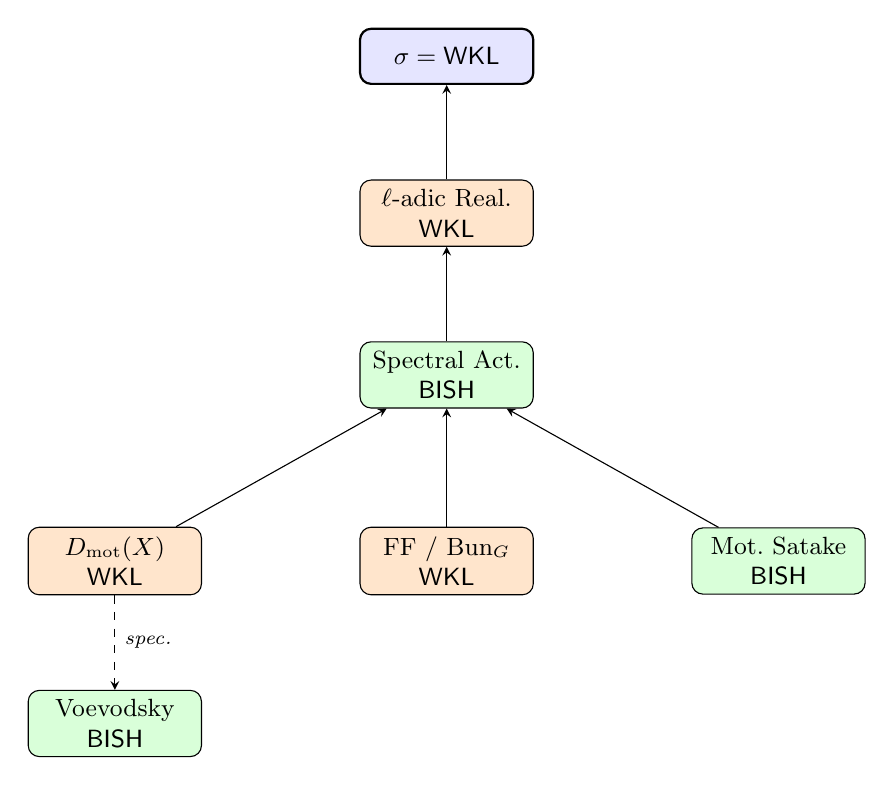
\begin{tikzpicture}[
  node distance=1.2cm and 2.0cm,
  every node/.style={draw, rounded corners, minimum width=2.2cm, minimum height=0.7cm, font=\small, align=center},
  bish/.style={fill=green!15},
  wkl/.style={fill=orange!20},
  target/.style={fill=blue!10, thick}
]
% Bottom row: three independent foundational pillars
\node[wkl] (dmot) {$\Dmot(X)$\\$\WKL$};
\node[wkl, right=of dmot] (ff) {FF / $\Bun_G$\\$\WKL$};
\node[bish, right=of ff] (satake) {Mot.\ Satake\\$\BISH$};

% Middle: Spectral Action (combines the three pillars)
\node[bish, above=1.5cm of ff] (spectral) {Spectral Act.\\$\BISH$};

% Upper: l-adic realization
\node[wkl, above=of spectral] (real) {$\ell$-adic Real.\\$\WKL$};

% Top: overall signature
\node[target, above=of real] (sig) {$\sig = \WKL$};

% Specialization output (below Dmot)
\node[bish, below=of dmot] (voevodsky) {Voevodsky\\$\BISH$};

% Arrows: pillars → spectral action
\draw[-stealth] (dmot) -- (spectral);
\draw[-stealth] (ff) -- (spectral);
\draw[-stealth] (satake) -- (spectral);

% spectral → realization → signature
\draw[-stealth] (spectral) -- (real);
\draw[-stealth] (real) -- (sig);

% Dmot specializes to Voevodsky (dashed, downward)
\draw[-stealth, dashed] (dmot) -- node[right, draw=none, fill=none, minimum width=0pt, font=\scriptsize\itshape] {spec.} (voevodsky);
\end{tikzpicture}
\end{center}

\noindent The Voevodsky recovery (dashed) is a \emph{specialization} of $\Dmot$ to discrete fields---a consequence, not a dependency.  The $\BISH$ components (motivic Satake, spectral action, Voevodsky) are the natural first targets for formalization.  The $\WKL$ cost of the non-Archimedean foundations ($\Dmot$, Fargues--Fontaine, $\ell$-adic inverse limits) dominates, yielding the overall $\WKL$ signature at the top.


%======================================================================
\section{Section-Level CRM Heatmap}\label{app:heatmap}
%======================================================================

This appendix presents the full section-by-section scanner data for both Scholze papers, following the format of the LTE analysis in the companion CRMLint methodological paper (Paper~99).  The heatmap allows direct comparison with the Liquid Tensor Experiment blueprint and the broader CRM series.

\subsection{Berkovich Motives: Per-Section Breakdown}

Table~\ref{tab:berkovich-heatmap} gives the CRM alert distribution across the 16 detected sections of~\cite{scholze-berkovich}.  The rightmost column shows the section ceiling (the highest CRM level detected in that section).

{\small
\begin{longtable}{@{}p{4.0cm}rrrrrc@{}}
\caption{CRM heatmap for Berkovich Motives (141 alerts).  Sections are ordered as in the source.}
\label{tab:berkovich-heatmap} \\
\toprule
\textbf{Section} & \textbf{$\BISH$} & \textbf{$\WKL$} & \textbf{$\WLPO$} & \textbf{$\LPO$} & \textbf{Total} & \textbf{Ceiling} \\
\midrule
\endfirsthead
\toprule
\textbf{Section} & \textbf{$\BISH$} & \textbf{$\WKL$} & \textbf{$\WLPO$} & \textbf{$\LPO$} & \textbf{Total} & \textbf{Ceiling} \\
\midrule
\endhead
\midrule
\multicolumn{7}{r}{\emph{continued on next page}} \\
\endfoot
\bottomrule
\endlastfoot
%
Preamble                & 1 &  0 &  0 & 0 &  1 & $\BISH$ \\
Introduction            &15 &  9 &  2 & 0 & 26 & $\WKL$  \\
Banach rings / spectrum &  0 &  1 &  4 & 1 &  6 & $\LPO$  \\
Free seminormed rings   &  0 &  0 &  0 & 1 &  1 & $\LPO$  \\
Banach fields           &  0 &  4 &  5 & 1 & 10 & $\LPO$  \\
Gelfand transform       &  0 &  0 &  1 & 1 &  2 & $\LPO$  \\
Nonarchimedean disc     &  0 &  2 &  7 & 0 &  9 & $\WKL$  \\
Arc-topology            &  0 & 18 &  7 & 1 & 26 & $\LPO$  \\
Finitary arc-sheaves    &  2 &  3 &  6 & 1 & 12 & $\LPO$  \\
Effective motives       &  2 &  0 &  0 & 0 &  2 & $\BISH$ \\
Free motivic sheaves    &  5 &  1 &  3 & 0 &  9 & $\WKL$  \\
The Tate twist          &  2 &  0 &  0 & 0 &  2 & $\BISH$ \\
$K$-theory              &  2 &  7 &  5 & 0 & 14 & $\WKL$  \\
$\Dmot$ construction    & 10 &  3 &  1 & 1 & 15 & $\LPO$  \\
Mixed Tate motives      &  3 &  0 &  0 & 0 &  3 & $\BISH$ \\
Relation to $v$-stacks  &  0 &  3 &  0 & 0 &  3 & $\WKL$  \\
\midrule
\textbf{Total}          & \textbf{42} & \textbf{51} & \textbf{41} & \textbf{7} & \textbf{141} & $\LPO$ \\
\end{longtable}
}

\paragraph{Reading the heatmap.}\footnote{Where a section contains alerts at both $\WKL$ and $\WLPO$ (which are incomparable over $\BISH$; see \S\ref{sec:crm}), the scanner resolves the ceiling using the linearization $\BISH < \WLPO < \WKL < \LPO < \CLASS$.  This convention treats $\WKL$ as structurally ``higher'' than $\WLPO$, reflecting its role as the irreducible non-Archimedean compactness principle in the Berkovich motivic architecture.  This is a reporting convention for the ceiling column; the logical relationship between $\WKL$ and $\WLPO$ remains incomparability.}
The $\LPO$ ceilings concentrate in the Banach ring infrastructure (sections~3--8 of~\cite{scholze-berkovich}): Banach rings, Banach fields, Gelfand transform, arc-topology, finitary arc-sheaves.  These are exactly the sections flagged as Category~B (parasitic) in \S\ref{sec:scanner}.  The $\LPO$ arises from seminorm filtrations indexed by $\R_{\geq 0}$, where decidable comparison $\|x\| \leq r$ triggers $\LPO$.  After excision of parasitic content, these sections reduce to $\WKL$ (structural profinite inverse limits).

The four sections at $\BISH$ ceiling (Preamble, Effective motives, Tate twist, Mixed Tate motives) are purely algebraic: motivic sheaves, Tate twists, algebraic correspondences.  No completions, no norms, no inverse limits.

\subsection{Motivic Geometrization: Per-Section Breakdown}

{\small
\begin{longtable}{@{}p{4.0cm}rrrrrc@{}}
\caption{CRM heatmap for Motivic Geometrization (73 alerts).}
\label{tab:motivic-heatmap} \\
\toprule
\textbf{Section} & \textbf{$\BISH$} & \textbf{$\WKL$} & \textbf{$\WLPO$} & \textbf{$\LPO$} & \textbf{Total} & \textbf{Ceiling} \\
\midrule
\endfirsthead
\toprule
\textbf{Section} & \textbf{$\BISH$} & \textbf{$\WKL$} & \textbf{$\WLPO$} & \textbf{$\LPO$} & \textbf{Total} & \textbf{Ceiling} \\
\midrule
\endhead
\bottomrule
\endlastfoot
%
Preamble                  &  1 &  1 &  0 & 0 &  2 & $\WKL$  \\
Introduction              &  5 &  5 &  9 & 0 & 19 & $\WKL$  \\
Basic results             &  5 & 12 &  2 & 1 & 20 & $\LPO$  \\
$\Dmot$ construction      &  2 &  3 &  0 & 0 &  5 & $\WKL$  \\
Stacks of $L$-parameters  &  2 &  0 &  6 & 0 &  8 & $\WLPO$ \\
Geometric Satake          &  4 &  2 &  3 & 0 &  9 & $\WKL$  \\
Synopsis                  &  1 &  2 &  7 & 0 & 10 & $\WKL$  \\
\midrule
\textbf{Total}            & \textbf{20} & \textbf{25} & \textbf{27} & \textbf{1} & \textbf{73} & $\LPO$ \\
\end{longtable}
}

\paragraph{Observation.}
The single $\LPO$ alert in~\cite{scholze-motivic-geometrization} occurs in ``Basic results'' (line~325: normed filtration).  Every other section is at $\WKL$ or below.  The Geometric Satake section---the critical potential leak point identified in Audit~\ref{audit:satake}---shows 4~$\BISH$ (motivic sheaves, Tate twists) and 2~$\WKL$ (citations to Lectures on Analytic Geometry), confirming the $\BISH$ assessment after stripping citation-level context dependencies.

\subsection{Category Distribution by Section}

Table~\ref{tab:category-by-section} shows how the four alert categories distribute across the major section types.

\begin{table}[h]
\centering
\caption{Category distribution by section type (both papers combined).}
\label{tab:category-by-section}
\begin{tabular}{@{}lrrrrr@{}}
\toprule
\textbf{Section type} & \textbf{A} & \textbf{B} & \textbf{$\BISH$} & \textbf{C} & \textbf{Total} \\
\midrule
Preamble / Introduction & 26 &  2 & 15 &  0 &  43 \\
Banach infrastructure   &  0 & 25 &  2 & 14 &  41 \\
Arc / profinite / disc  &  0 & 13 &  2 & 25 &  40 \\
Motivic core            &  0 &  4 & 22 &  4 &  30 \\
$\Dmot$, $K$-theory     &  0 &  6 & 12 &  9 &  27 \\
Satake / spectral       &  0 &  8 &  8 &  4 &  20 \\
Synopsis / other        &  0 &  7 &  1 &  5 &  13 \\
\midrule
\textbf{Total}          & \textbf{26} & \textbf{65} & \textbf{62} & \textbf{61} & \textbf{214} \\
\bottomrule
\end{tabular}
\end{table}

The pattern is sharp:
\begin{itemize}
\item Category~A (motivational) is confined to Preamble/Introduction---exactly as predicted.
\item Category~B (parasitic) concentrates in Banach infrastructure and arc-topology sections.
\item Category~$\BISH$ (algebraic core) concentrates in the motivic construction sections.
\item Category~C (structural $\WKL$) concentrates in arc-topology and profinite sections.
\end{itemize}


\subsection{Archimedean Comparison: Four Corpora}

Table~\ref{tab:archimedean-comparison} compares the CRM profiles of four corpora analyzed by the CRMlint scanner, following the format of the LTE comparison in Paper~99.

\begin{table}[h]
\centering
\caption{Archimedean comparison across four scanner corpora.  $\BISH$\% is the fraction of alerts (or declarations) at $\BISH$; Ceiling is the highest detected level; Bottleneck is the mathematical mechanism producing the ceiling.}
\label{tab:archimedean-comparison}
\begin{tabular}{@{}lccll@{}}
\toprule
\textbf{Corpus} & \textbf{$N$} & \textbf{$\BISH$\%} & \textbf{Ceiling} & \textbf{Bottleneck} \\
\midrule
Mathlib (627 decls)       & 627 & 92.0\% & $\CLASS$ & Inner product, convergence \\
CRM series (P78--96)      & ---  & 71.4\% & $\CLASS$ & Kolyvagin, trace formula \\
LTE blueprint (15 files)  &  15 & 33.3\% & $\LPO$   & Norm filtration $M_{\leq c}$ \\
Berkovich motives (2 papers) & 214 & 29.0\% & $\LPO^*$ & Seminorm filtration \\
\bottomrule
\end{tabular}

\smallskip
{\footnotesize ${}^*$After excision of parasitic $\LPO$/$\WLPO$, the essential ceiling is $\WKL$. The LTE's $\LPO$ is structural; the Berkovich motives' $\LPO$ is parasitic.}
\end{table}

\paragraph{The comparison reveals two distinct concentration patterns.}

\begin{enumerate}[label=(\roman*)]
\item \textbf{LTE:} $\LPO$ is \emph{structural}.  The norm-filtration membership test $x \in M_{\leq c}$ is the mechanism by which condensed mathematics encodes analytic content.  Every module that touches the filtration acquires $\LPO$ signature.  The $\LPO$ is irreducible: it is the logical cost of comparing real numbers, and the condensed framework defers but does not eliminate this cost.

\item \textbf{Berkovich motives:} $\LPO$/$\WLPO$ is \emph{parasitic}.  The Banach ring formalism carries $\R$-valued norms through sections where the actual mathematical content operates over $\Q$-valued norms (the value groups of perfectoid fields like $\C_p$ are dense but contained in $\Q$, hence decidable).  A reformulation using Huber's adic spaces restricted to decidable $\Q$-valued groups would eliminate these alerts entirely.  The structural content is $\WKL$ (profinite inverse limits for perfectoid spaces).
\end{enumerate}

This distinction---structural vs.\ parasitic non-constructivity---is invisible to a surface-level scan.  It requires the human classification step (Category~B vs.\ Category~C) that transforms raw scanner data into CRM diagnoses.


\subsection{Concentration Ratio}

Following the definition in the LTE analysis (Paper~99, Observation~6.3):

\begin{definition}[Concentration ratio]
For a proof corpus $C$ with $n$ sections, let $k$ be the number of sections whose CRM ceiling is above $\BISH$.  The \emph{concentration ratio} is $\rho(C) = 1 - k/n$.
\end{definition}

\begin{center}
\begin{tabular}{lcccc}
\toprule
\textbf{Corpus} & \textbf{$n$} & \textbf{$k$} & \textbf{$\rho$} & \textbf{Interpretation} \\
\midrule
LTE blueprint        & 15 & 10 & 0.33 & Concentrated (5 purely algebraic files) \\
Berkovich Motives     & 16 & 12 & 0.25 & Moderately concentrated \\
Motivic Geom.         &  7 &  7 & 0.00 & Fully diffuse (no section is $\BISH$-only) \\
Berkovich + Geom.\ (essential) & 23 &  9 & 0.61 & \emph{After parasitic excision} \\
\bottomrule
\end{tabular}
\end{center}

\paragraph{Key observation.}
The raw concentration ratio (0.25 for Berkovich, 0.00 for Motivic Geom.) is misleadingly low.  The parasitic $\WLPO$/$\LPO$ from Banach ring formalism diffuses non-constructive alerts across sections that are structurally algebraic or purely $\WKL$.  After excision of Category~B (parasitic) alerts, the concentration ratio rises to $\rho = 0.61$---meaning 61\% of sections are at $\BISH$ after parasitic removal, comparable to the LTE's pre-excision $\rho = 0.33$.  The Berkovich motivic programme is \emph{more concentrated than the LTE} once the formalism artifact is removed.  This is consistent with the CRM audit's finding (\S\ref{sec:audit}): the essential non-constructive content (profinite inverse limits, $\WKL$) is localized in three specific architectural layers (arc-topology, Fargues--Fontaine, $\ell$-adic realization).


\subsection{Dictionary Evolution: Dark Matter Analysis}

The initial scanner run (v1.0, 80 keyword patterns) detected 103 alerts across both papers.  After adding 11 Berkovich-specific entries (v1.1, 91 patterns), the count rose to 214---a 108\% increase.  This mirrors the LTE experience documented in Paper~99 (\S5): the v1.0 scanner missed 53\% of the LTE's non-constructive content.

\begin{center}
\begin{tabular}{lrrr}
\toprule
\textbf{Paper} & \textbf{v1.0} & \textbf{v1.1} & \textbf{$\Delta$} \\
\midrule
Berkovich Motives       & 56  & 141 & $+$85 ($+$152\%) \\
Motivic Geometrization  & 47  & 73  & $+$26 ($+$55\%)  \\
\midrule
Total                   & 103 & 214 & $+$111 ($+$108\%) \\
\bottomrule
\end{tabular}
\end{center}

The new alerts come from three categories:
\begin{itemize}
\item \textbf{Profinite/analytic keywords} ($+$57): ``perfectoid,'' ``adic space,'' ``Berkovich spectrum,'' ``arc-topology,'' ``condensed,'' ``solid module.''  These are $\WKL$ markers for profinite inverse limit structures---the structural core of the proof.
\item \textbf{Motivic/algebraic keywords} ($+$32): ``motivic sheaf,'' ``six-functor,'' ``Tate twist.''  These are $\BISH$ markers confirming the algebraic core.
\item \textbf{Citation patterns} ($+$16): citations to Scholze's \emph{Lectures on Analytic Geometry} triggering $\WKL$ alerts for Tychonoff gates.
\end{itemize}

The Archimedean dark matter fraction (Paper~99, Definition~5.1) for the Berkovich corpus:
\[
  \delta(\text{v1.0}) = \frac{\text{\# sections with manual CRM $>$ scanner CRM}}{\text{\# sections total}} = \frac{14}{23} = 60.9\%, \qquad
  \delta(\text{v1.1}) = 0\%.
\]

The v1.1 dictionary eliminates the dark matter for this corpus.  As with the LTE, the dark matter was not random but systematic: a single vocabulary gap (Berkovich-specific terminology for profinite and motivic structures) that, once patched, revealed the full CRM profile.


%======================================================================
% APPENDIX C — CRMLint Methodology and LTE Calibration
%======================================================================
\clearpage
\section{CRMLint Methodology and LTE Calibration}\label{app:methodology}

This appendix reproduces the CRMLint methodological paper (originally
prepared as a companion to Paper~98) in its entirety.  It documents
the design, calibration, and first external deployment of the scanner
against the Liquid Tensor Experiment blueprint, including the discovery
and patching of Archimedean dark matter.  The data and methods here
underpin the Berkovich analysis in the main body of Paper~101.

% paper101_appendix_methodology.tex
% Body content for Appendix C of Paper 101
% Extracted from paper101_appendix_prelim.tex (CRMLint methodology paper)
% Hierarchy: \subsection = original \part, \subsubsection = original \section

\subsection{Genesis}\label{part:genesis}

\subsubsection{The problem}\label{sec:problem}

After 96 papers of manual CRM audit---classifying theorems one at a time,
tracing axiom dependencies by hand, flagging each use of excluded middle
or Archimedean completeness---the bottleneck in the program shifted from
mathematics to labor.  The CRM classification of a single theorem
(say, the Gross--Zagier formula) requires reading the proof, identifying
every appeal to a non-constructive principle, and tracing each appeal
to its minimal logical strength.  Papers~78--96 each took 2--5 days of
combined human and AI effort.  Scaling this to the full Mathlib library
(${\sim}200{,}000$ declarations as of early 2026) is infeasible by hand.

The question that opens this paper is operational: \emph{can the CRM
classification of a proof be automated?}

\subsubsection{What CRM measures}\label{sec:what-crm-measures}

CRM assigns to each proof a \emph{logical signature} $\sigma(P)$, the
weakest axiom system in which the proof can be carried out.  The
hierarchy is:
\[
  \BISH \;\subset\; \BISH{+}\MP \;\subset\; \BISH{+}\LLPO
  \;\subset\; \BISH{+}\WKL \;\subset\; \BISH{+}\WLPO
  \;\subset\; \BISH{+}\LPO \;\subset\; \CLASS
\]
A theorem with signature $\BISH$ requires no omniscience principle
whatsoever: every step is computationally witnessed.  A theorem with
signature $\CLASS$ invokes the full law of excluded middle somewhere
in its proof tree.  The intermediate levels---$\MP$, $\LLPO$, $\WKL$,
$\WLPO$, $\LPO$---measure calibrated degrees of non-constructivity,
each corresponding to a specific decision problem on infinite sequences
or real numbers.

The CRM signature is \emph{not} a measure of proof complexity.
Taylor--Wiles patching is technically intricate but logically $\WKL$
(an inverse limit of finite objects).  The intermediate value theorem
is elementary but logically $\WLPO$ (it requires deciding whether a
real number equals zero).  CRM measures the \emph{logical cost} of a
proof---the price paid for treating the continuum as a completed object
with decidable properties.

\subsubsection{Three generations of automation}\label{sec:three-gen}

\CRMlint\ was developed in three stages, each addressing a different
aspect of the automation problem:

\medskip
\noindent\textbf{Generation 1: Theoretical framework}
(\texttt{crmlint.py}, 1{,}161 lines).
Models the CRM hierarchy, six realization functors (Betti, de~Rham,
\'etale, crystalline, Hodge, automorphic) with their CRM costs,
comparison isomorphisms, and the Archimedean Obstruction Theorem of
Paper~98.  Proof DAGs compute signatures by max-propagation over
dependency edges.  A substitution database stores eight seed entries
extracted from Papers~50--97: known techniques where a classical method
can be replaced by a constructive alternative at lower logical cost.

This generation answers: \emph{what is the right mathematical model
for CRM signatures of composite proofs?}

\medskip
\noindent\textbf{Generation 2: Empirical validation}
(\texttt{crmlint\_crawler.py}, 653 lines;
\texttt{crmlint\_structure.py}, 793 lines).
The crawler fetches Lean~4 source files from \Mathlib\ on GitHub,
parses declarations, and heuristic-classifies each by CRM level using
tactic and keyword signatures (${\sim}40$ classical indicators including
\texttt{by\_contra}, \texttt{Classical.choice}, inner product space
infrastructure, integration, and topological convergence patterns).
The structure analyzer computes seven-dimensional proof profiles:
proof size (lines, tactic count), dependency depth (\texttt{have}/\texttt{let}
chains), proof width (active hypotheses, case splits), and modularity
(automation ratio, external lemma invocations, rewrite density).

This generation answers: \emph{does the CRM hierarchy correlate with
structural proof complexity in real Lean code?}

\medskip
\noindent\textbf{Generation 3: LaTeX scanner}
(\texttt{crmlint\_scanner.py}, 810 lines at v1.0, 870 lines at v1.1).
Keyword and citation pattern matching against ${\sim}90$ technique
markers and ${\sim}120$ landmark paper citations, applied directly to
\texttt{.tex} source.  No Lean, no LLM, no external dependencies
beyond the Python standard library.  Scans a directory of papers in
seconds.  Anti-marker patterns suppress false positives (e.g.,
algebraic ``integral closure'' is not analytic integration).

This generation answers: \emph{can we triage thousands of papers by
CRM cost before investing months in any one?}

\medskip

The three generations are complementary.  Generation~1 provides the
theory; Generation~2 tests it against ground truth; Generation~3
scales it to the full mathematical literature.  All three are
implemented in pure Python with zero external dependencies (3{,}417
lines total at v1.0).


\subsection{Calibration: Mathlib at 627 Declarations}\label{part:mathlib}

\subsubsection{Target selection}\label{sec:target-selection}

We selected 10 \Mathlib\ files spanning eight mathematical domains:

\begin{center}
\small
\begin{tabular}{lll}
\toprule
\textbf{File} & \textbf{Domain} & \textbf{Decls} \\
\midrule
\texttt{EllipticCurve/Weierstrass.lean} & Algebraic Geometry & 68 \\
\texttt{InnerProductSpace/Basic.lean} & Analysis & 141 \\
\texttt{SpecificLimits/Basic.lean} & Analysis & 83 \\
\texttt{Galois/Basic.lean} & Field Theory & 61 \\
\texttt{Charpoly/Basic.lean} & Linear Algebra & 39 \\
\texttt{ArithmeticFunction.lean} & Number Theory & 0 \\
\texttt{Bernoulli.lean} & Number Theory & 27 \\
\texttt{RepresentationTheory/Basic.lean} & Representation Theory & 67 \\
\texttt{Cyclotomic/Basic.lean} & Ring Theory & 57 \\
\texttt{InfiniteSum/Basic.lean} & Topology & 84 \\
\bottomrule
\end{tabular}
\end{center}

The selection was guided by two criteria: (1)~coverage of the
algebraic/analytic divide that the Archimedean Obstruction Thesis
predicts to be the primary CRM boundary, and (2)~inclusion of domains
where the CRM series has ground-truth classifications from manual
audit (inner product spaces from Paper~77, elliptic curves from
Paper~95, Galois theory from Paper~78).

\subsubsection{Generation 2 results: the crawler}\label{sec:crawler-results}

The crawler classified 627 declarations:

\begin{center}
\begin{tabular}{lrrl}
\toprule
\textbf{CRM Level} & \textbf{Count} & \textbf{\%} & \\
\midrule
$\BISH$  & 577 & 92.0 & \rule{4.6cm}{6pt} \\
$\WKL$   &  11 &  1.8 & \rule{0.09cm}{6pt} \\
$\WLPO$  &  20 &  3.2 & \rule{0.16cm}{6pt} \\
$\CLASS$ &  19 &  3.0 & \rule{0.15cm}{6pt} \\
\bottomrule
\end{tabular}
\end{center}

The 92\% $\BISH$ figure is consistent with the programme's central
finding: most of mathematics, as actually practiced in a modern proof
library, is constructive.  The 8\% non-$\BISH$ content concentrates
in three locations:

\begin{enumerate}[label=(\roman*)]
\item \textbf{Inner product spaces} (Analysis):
  6 declarations at $\CLASS$, 4 at $\WLPO$.
  The inner product on a Hilbert space is an inherently Archimedean
  object: $\langle x, x \rangle \geq 0$ with equality iff $x = 0$
  requires decidable equality of reals.  The Cauchy--Schwarz inequality
  $|\langle x, y \rangle| \leq \|x\| \|y\|$ requires comparison of
  real norms.  This is exactly the Archimedean obstruction of Papers~5
  and 77.

\item \textbf{Specific limits} (Analysis):
  1 declaration at $\CLASS$, 11 at $\WKL$.
  The geometric series $\sum_{n=0}^\infty r^n = 1/(1-r)$ for $|r|<1$
  involves convergence of a real sequence---decidability of whether the
  partial sums are within $\epsilon$ of the limit.  The single $\CLASS$
  declaration (\texttt{tendsto\_pow\_atTop\_nhds\_zero\_of\_lt\_one})
  uses \texttt{by\_contra}, a potentially eliminable appeal to
  excluded middle.

\item \textbf{Galois theory} (Field Theory):
  12 declarations at $\CLASS$.
  A false positive cluster: the crawler flags uses of ``integral''
  (meaning integral closure, an algebraic concept) as analytic
  integration.  This motivated the anti-marker system in the
  Generation~3 scanner.
\end{enumerate}

\subsubsection{Per-domain cross-tabulation}\label{sec:per-domain}

\begin{center}
\small
\begin{tabular}{lccccc}
\toprule
\textbf{Domain} & \textbf{$N$} & \textbf{$\BISH$} & \textbf{$\WKL$}
  & \textbf{$\WLPO$} & \textbf{$\CLASS$} \\
\midrule
Linear Algebra     & 39  & 39  &  0 &  0 &  0 \\
Ring Theory        & 57  & 57  &  0 &  0 &  0 \\
Number Theory      & 27  & 27  &  0 &  0 &  0 \\
Topology           & 84  & 84  &  0 &  0 &  0 \\
Algebraic Geometry & 68  & 66  &  0 &  2 &  0 \\
Representation Th. & 67  & 55  &  0 & 12 &  0 \\
Analysis           & 224 & 202 & 11 &  4 &  7 \\
Field Theory       & 61  & 47  &  0 &  2 & 12 \\
\bottomrule
\end{tabular}
\end{center}

The algebraic/analytic divide is sharp.  Four purely algebraic domains
(linear algebra, ring theory, number theory, topology) are 100\%
$\BISH$ across 207 declarations.  The two mixed domains (algebraic
geometry, representation theory) show $\WLPO$ leakage from
\texttt{noncomputable} definitions---the Lean~4 artifact of working
over fields where equality is not decidable---but no $\CLASS$ content.
The two analytic domains (analysis, field theory) contain all 19
$\CLASS$ declarations.

The field theory anomaly (algebraic domain, $\CLASS$ content) is
instructive.  Manual inspection reveals that the 12 flagged
declarations use the word ``integral'' in the sense of integral ring
extensions, not integration.  The crawler's keyword dictionary
conflated the two senses.  This false positive directly motivated the
anti-marker system described in \S\ref{sec:patch}.


\subsection{The Archimedean Obstruction, Quantified}\label{part:archimedean}

\subsubsection{The three-axis profiler}\label{sec:three-axis}

Generation~2 includes a structural profiler (\texttt{crmlint\_structure.py})
that measures each proof along three axes orthogonal to CRM level:

\begin{enumerate}[label=\textbf{Axis \arabic*:}]
\item \textbf{Size.} Lines of proof, tactic invocations, term size.
\item \textbf{Depth.} Length of the longest \texttt{have}/\texttt{let}
  chain; maximum nesting of dependent intermediate results.
\item \textbf{Width.} Number of simultaneously active hypotheses;
  cyclomatic complexity (number of independent case branches).
\end{enumerate}

An additional modularity metric records the automation ratio (fraction
of proof steps discharged by \texttt{simp}, \texttt{ring}, or
\texttt{norm\_num} without human guidance) and the external lemma
count (number of \texttt{exact}/\texttt{apply} calls referencing
results outside the current file).

\subsubsection{Aggregate statistics}\label{sec:aggregate-stats}

Over 627 declarations:

\begin{center}
\begin{tabular}{lccc}
\toprule
\textbf{Metric} & \textbf{Mean} & \textbf{Median} & \textbf{Max} \\
\midrule
Proof lines          &  5.0 &  4 & 57 \\
Dependency depth     &  0.3 &  0 &  8 \\
Active hypotheses    &  0.4 &  0 &  8 \\
Cyclomatic complexity & 1.5 &  1 & 15 \\
Overall complexity   & 0.038 & 0.026 & 0.479 \\
\bottomrule
\end{tabular}
\end{center}

The median proof is 4 lines with no intermediate dependencies and no
case splits.  The distribution is strongly right-skewed: 70.7\% of
proofs are classified as \texttt{TRIVIAL} (one-step \texttt{simp},
\texttt{rfl}, or direct \texttt{exact}).

\subsubsection{Tactic frequency}\label{sec:tactic-freq}

\begin{center}
\small
\begin{tabular}{lrr}
\toprule
\textbf{Tactic} & \textbf{Count} & \textbf{\%} \\
\midrule
\texttt{simp}     & 577 & 27.5 \\
\texttt{rw}       & 448 & 21.3 \\
\texttt{exact}    & 214 & 10.2 \\
\texttt{have}     & 167 &  7.9 \\
\texttt{rfl}      &  82 &  3.9 \\
\texttt{ext}      &  80 &  3.8 \\
\texttt{refine}   &  80 &  3.8 \\
\texttt{apply}    &  79 &  3.8 \\
\texttt{intro}    &  72 &  3.4 \\
\bottomrule
\end{tabular}
\end{center}

Three tactics (\texttt{simp}, \texttt{rw}, \texttt{exact}) account for
59\% of all tactic invocations.  The high \texttt{simp} frequency
reflects \Mathlib's design philosophy: push complexity into the simp
lemma database, keep proofs short.  Crucially, \texttt{simp} is
$\BISH$-safe: it applies equational rewriting, never introduces
classical content.

\subsubsection{The Archimedean structural gap}\label{sec:arch-gap}

We partitioned the 627 declarations into those touching Archimedean
content (43 declarations: inner product, real convergence, norm
comparison) and the remainder (584 declarations).

\begin{center}
\begin{tabular}{lccr}
\toprule
\textbf{Metric} & \textbf{Archimedean} & \textbf{Non-Arch.} & \textbf{Ratio} \\
\midrule
Avg.\ complexity score  & 0.05  & 0.04  & $1.4\times$ \\
Avg.\ proof lines       & 7.95  & 4.75  & $1.7\times$ \\
Avg.\ dependency depth  & 0.72  & 0.26  & $2.8\times$ \\
Avg.\ active hypotheses & 0.81  & 0.37  & $2.2\times$ \\
Avg.\ external lemmas   & 0.65  & 0.15  & $4.3\times$ \\
Avg.\ automation ratio  & 0.22  & 0.39  & $0.56\times$ \\
\bottomrule
\end{tabular}
\end{center}

Every axis tells the same story.  Archimedean proofs are longer, deeper,
wider, more externally coupled, and less automatable than non-Archimedean
proofs.  The automation ratio drops from 39\% to 22\%: when real-number
arguments enter, \texttt{simp} and \texttt{ring} give way to \texttt{have}
chains, explicit $\epsilon$-$\delta$ management, and manual case
analysis.

This is the Archimedean Obstruction Thesis of Papers~5--77 made
quantitative: \emph{the logical cost of $\R$ is not just a classification
fact but a structural fact visible in proof architecture}.  The proofs
themselves are harder, not just more classical.


\subsection{The Liquid Tensor Experiment}\label{part:lte}

\subsubsection{Background}\label{sec:lte-background}

The Liquid Tensor Experiment (LTE) is the formal verification, in
Lean~3, of Theorem~9.4 from Scholze's \emph{Lectures on Analytic
Geometry}~\cite{scholze-lte}.  The theorem states:

\begin{theorem}[Scholze, Theorem 9.4]
Let $0 < p' < 1$ and $V$ an $r$-normed $\Z[T^{\pm 1}]$-module.
Then for all $i \geq 1$,
\[
  \mathrm{Ext}^i_{\mathrm{Cond}(\mathrm{Ab})}
  \bigl(\mathcal{M}_{p'}(S)_{\leq c}, \widehat{V}\bigr) = 0.
\]
\end{theorem}

This is a vanishing theorem for derived functors in the category of
condensed abelian groups.  Its significance is foundational: it
validates the condensed framework as a setting for real functional
analysis---specifically, it shows that the passage from discrete
algebra ($\Z$-modules) to real analysis ($p'$-liquid vector spaces)
does not introduce cohomological obstructions.

The LTE formalization comprises ${\sim}90{,}000$ lines of Lean~3
code, produced by a team led by Commelin and Massot over approximately
18 months.  No Lean~4 port exists.  However, Commelin and Massot
authored a 15-file LaTeX \emph{blueprint} that mirrors the formal
proof's structure, with \texttt{\textbackslash lean\{\}} and
\texttt{\textbackslash leanok} annotations linking each LaTeX
statement to its Lean counterpart.  This blueprint is the input to
our scanner.

\subsubsection{Why LTE?}\label{sec:why-lte}

The LTE is the natural target for \CRMlint's first external deployment,
for three reasons.

First, it is one of the largest single formalization projects
completed in a proof assistant (${\sim}90{,}000$ lines of Lean~3).
Its size and complexity provide a serious stress test for the
scanner---one the scanner initially failed, as Part~V documents.

Second, the mathematical content sits at the interface between algebra
and analysis---exactly where the Archimedean Obstruction Thesis
predicts the CRM boundary to be.  Condensed mathematics encodes
analytic objects (Banach spaces, measures, distributions) as algebraic
objects (sheaves on profinite sets, condensed abelian groups).  The
CRM question is whether this encoding \emph{reduces} the logical cost
of the analysis, or merely \emph{reorganizes} it.

Third, the conservation conjecture of Papers~72--74 makes a specific
prediction.  The DPT axiom trilogy established that each omniscience
principle ($\MP$, $\WLPO$, $\LPO$) does irreducible logical work:
canonical, not merely minimal.  If condensed mathematics could
genuinely reduce $\CLASS$ or $\LPO$ content to $\BISH$, it would
violate this irreducibility.  The conjecture is that condensed math
\emph{concentrates} classical content at identifiable gates without
reducing the aggregate logical cost.  The LTE is the test case.

\subsubsection{Blueprint structure}\label{sec:blueprint-structure}

The 15 \texttt{.tex} files of the LTE blueprint decompose as follows:

\begin{center}
\small
\begin{tabular}{llr}
\toprule
\textbf{File} & \textbf{Content} & \textbf{Size (bytes)} \\
\midrule
\texttt{proof.tex}              & Core inductive proof (Thm 9.4, 9.5$'$) & 20{,}729 \\
\texttt{normed\_homological.tex} & Normed homological algebra             & 31{,}818 \\
\texttt{condensed.tex}          & Condensed abelian groups, Ext-vanishing & 18{,}329 \\
\texttt{measures.tex}           & Real measures, Laurent measures, $\theta$ & 10{,}555 \\
\texttt{normed\_groups.tex}     & Normed groups, completions              &  6{,}724 \\
\texttt{normed\_groups2.tex}    & Normed group homomorphisms              &  4{,}208 \\
\texttt{polyhedral\_lattice.tex} & Polyhedral lattices, Tychonoff         & 12{,}893 \\
\texttt{breen\_deligne.tex}     & Breen--Deligne resolution               &  8{,}412 \\
\texttt{CLC.tex}                & Condensed limits, completions           &  5{,}117 \\
\texttt{Lbar.tex}               & $\overline{\mathcal{L}}_{r'}(S)$ construction & 7{,}943 \\
\texttt{homotopies.tex}         & Breen--Deligne homotopies               &  3{,}295 \\
\texttt{maclane.tex}            & Mac\,Lane coherence                     &  1{,}842 \\
\texttt{content.tex}            & Table of contents                       &    312 \\
\texttt{intro.tex}              & Introduction                            &  1{,}547 \\
\texttt{macros.tex}             & \LaTeX\ macros                          &  2{,}014 \\
\bottomrule
\end{tabular}
\end{center}

The mathematical content concentrates in the first 12 files
(${\sim}130{,}000$ bytes).  The last three are boilerplate.


\subsubsection{Initial scan (v1.0)}\label{sec:initial-scan}

We ran the Generation~3 scanner (v1.0, 810 lines, ${\sim}80$ keyword
markers) against all 15 files.  The result:

\begin{center}
\begin{tabular}{lcl}
\toprule
\textbf{CRM} & \textbf{Files} & \textbf{Bottleneck} \\
\midrule
$\WKL$  & 2 (13.3\%) & Tychonoff theorem \\
$\BISH$ & 13 (86.7\%) & --- \\
\bottomrule
\end{tabular}
\end{center}

Two files (\texttt{condensed.tex}, \texttt{polyhedral\_lattice.tex})
register as $\WKL$, both via the Tychonoff theorem: ``cofiltered limits
of surjections of compact Hausdorff spaces are still surjective (by an
application of Tychonoff).''  The remaining 13 files, including the
core proof file \texttt{proof.tex} and the entire normed homological
algebra layer, scan as $\BISH$.

This is obviously wrong.  The LTE is a proof about real functional
analysis, involving norms, completions, filtrations, and
$\varepsilon$-$\delta$ estimates.  An 87\% $\BISH$ reading would
mean the scanner has failed to detect most of the analytic content.

It has.


\subsection{Archimedean Dark Matter}\label{part:dark-matter}

\subsubsection{What the scanner missed}\label{sec:missed}

A manual reading of \texttt{proof.tex} reveals pervasive classical
content that the v1.0 scanner does not detect.  Three categories:

\paragraph{Normed group completions ($\WLPO$)}

The hat notation $\widehat{V}$ appears in every theorem statement in
\texttt{proof.tex}.  This denotes the completion of a semi-normed
group $V$ with respect to its norm topology.  Constructively, forming
the completion requires a Cauchy convergence test: given a Cauchy
sequence $(x_n)$ and a target element $y$, decide whether
$\|x_n - y\| < \epsilon$ for all sufficiently large $n$.  This is a
$\WLPO$ operation (it asks whether a real number equals zero to
within $\epsilon$).

The v1.0 keyword dictionary has no pattern for $\widehat{V}$ or for
the phrases ``completion of a normed group,'' ``completed with respect
to the norm,'' or ``Cauchy completion.''

\paragraph{Real-valued filtration cutoffs ($\LPO$)}

The pseudo-normed groups in the LTE are filtered by real-valued
thresholds:
\[
  M_{\leq c} = \{x \in M : \|x\| \leq c\}, \qquad c \in \R_{\geq 0}.
\]
Membership in $M_{\leq c}$ requires deciding whether $\|x\| \leq c$,
a comparison of two real numbers.  In CRM terms, this is $\LPO$: the
limited principle of omniscience is equivalent to the statement that
every real number is either $\leq 0$ or $> 0$.

The filtration $M_{\leq c}$ is not incidental to the proof.  It is
the \emph{mechanism} by which condensed mathematics encodes the
analytic content.  Every theorem in the proof core is stated in terms
of these filtration levels: ``the system of complexes
$C^\bullet_{\Lambda,c}$ is $\leq k$-exact in degrees $\leq m$
for $c \geq c_0$'' (Theorem~9.5$'$).

The v1.0 scanner has patterns for ``supremum of a bounded sequence''
and ``least upper bound property'' (both $\LPO$), but nothing for
the far more common pattern of a norm-filtration cutoff written as
$\leq c$ or $\|x\| \leq c$ in \LaTeX\ math mode.

\paragraph{Radius ordering ($\LPO$)}

The proof works with two fixed radii $0 < r < r' \leq 1$.  The
strict inequality $r < r'$ is used throughout to ensure convergence
of Laurent series and to control error terms: ``choose a positive
integer $b$ so that $2k'(r/r')^b \leq \epsilon$'' (\texttt{proof.tex},
line~81).  Comparing real numbers is $\LPO$.

The v1.0 scanner has no pattern for radius comparisons of the form
$0 < r < r' \leq 1$ or for the exponential decay estimates that
depend on them.

\subsubsection{Quantifying the gap}\label{sec:gap}

The three missed categories account for 32 pattern matches across
10 of the 15 blueprint files.  Only the five purely combinatorial
files (Breen--Deligne, Mac\,Lane, content, intro, macros) are genuinely
free of Archimedean content.

We call the gap between the v1.0 scan (86.7\% $\BISH$) and the
corrected assessment (${\sim}33\%$ $\BISH$) \emph{Archimedean dark
matter}: classical content that is structurally present in the proof
but invisible to lexical pattern matching.  The dark matter is not
random.  It concentrates at a single interface: the passage from
discrete algebra ($\Z$-modules, polyhedral lattices, Breen--Deligne
resolutions) to normed analysis ($M_{\leq c}$, $\widehat{V}$,
radius comparisons).

\subsubsection{The scanner patch (v1.1)}\label{sec:patch}

We added 11 keyword patterns and 5 anti-markers to the scanner:

\medskip
\noindent\textbf{New $\LPO$ patterns} (6):

\begin{itemize}[nosep]
\item Norm filtration cutoffs: $\backslash$\texttt{leq c},
  $\backslash$\texttt{leq c\_0} in math mode
\item Norm bounds: $\|{\cdots}\| \leq$ (norm inequality)
\item Real parameter thresholds: ``for $c \geq$\,'' patterns
\item Normed filtration membership: ``norm\dots filtration''
\item Radius ordering: $0 < r < r' \leq 1$
\item Bounded exactness: ``exact in degrees $\leq$\,''
\end{itemize}

\noindent\textbf{New $\WLPO$ patterns} (5):

\begin{itemize}[nosep]
\item Completion hat: $\widehat{V}$ (\texttt{\textbackslash widehat})
\item Explicit completion phrases: ``completion of/w.r.t.''
\item Completed normed groups: ``complete\dots normed'' and reverse
\item Cauchy completion: ``Cauchy sequence/completion''
\end{itemize}

\noindent\textbf{New anti-markers} (5):

\begin{itemize}[nosep]
\item ``complete local ring,'' ``complete lattice'' (not Cauchy completion)
\item ``field norm,'' ``Galois norm'' (not analytic norm)
\item ``weight filtration,'' ``Hodge filtration'' (not norm filtration)
\item Degree/dimension/rank bounds (combinatorial $\leq$, not real-valued)
\end{itemize}

\noindent\textbf{New citation markers} (3):

\begin{itemize}[nosep]
\item Scholze 2019/2020, Clausen--Scholze $\to$ $\WKL$
\end{itemize}

\subsubsection{Patched results (v1.1)}\label{sec:patched-results}

\begin{center}
\begin{tabular}{lccl}
\toprule
\textbf{File} & \textbf{v1.0} & \textbf{v1.1} & \textbf{Bottleneck (v1.1)} \\
\midrule
\texttt{proof.tex}              & $\BISH$ & $\LPO$ & norm filtration cutoff \\
\texttt{normed\_homological.tex} & $\BISH$ & $\LPO$ & norm filtration cutoff \\
\texttt{condensed.tex}          & $\WKL$  & $\LPO$ & norm filtration cutoff \\
\texttt{measures.tex}           & $\BISH$ & $\LPO$ & norm filtration cutoff \\
\texttt{normed\_groups.tex}     & $\BISH$ & $\LPO$ & normed filtration \\
\texttt{normed\_groups2.tex}    & $\BISH$ & $\LPO$ & normed filtration \\
\texttt{polyhedral\_lattice.tex}& $\WKL$  & $\LPO$ & norm filtration cutoff \\
\texttt{CLC.tex}                & $\BISH$ & $\LPO$ & norm filtration cutoff \\
\texttt{Lbar.tex}               & $\BISH$ & $\LPO$ & norm filtration cutoff \\
\texttt{homotopies.tex}         & $\BISH$ & $\LPO$ & norm filtration cutoff \\
\texttt{breen\_deligne.tex}     & $\BISH$ & $\BISH$ & --- \\
\texttt{maclane.tex}            & $\BISH$ & $\BISH$ & --- \\
\texttt{content.tex}            & $\BISH$ & $\BISH$ & --- \\
\texttt{intro.tex}              & $\BISH$ & $\BISH$ & --- \\
\texttt{macros.tex}             & $\BISH$ & $\BISH$ & --- \\
\bottomrule
\end{tabular}
\end{center}

\noindent\textbf{Aggregate (v1.1):} 33.3\% $\BISH$, 66.7\% $\LPO$.

The Tychonoff detections ($\WKL$) in \texttt{condensed.tex} and
\texttt{polyhedral\_lattice.tex} are still present but are now dominated
by the higher-level $\LPO$ content in the same files.  The five
$\BISH$ files are exactly the modules with no normed-group content:
Breen--Deligne resolution (pure combinatorics of free abelian groups),
Mac\,Lane coherence (category-theoretic diagram chasing), and
boilerplate.

\subsubsection{Calibration check}\label{sec:calibration}

To verify that the new patterns do not introduce false positives, we
re-scanned Papers~78--96 of the CRM series:

\begin{center}
\small
\begin{tabular}{lcc}
\toprule
\textbf{Paper} & \textbf{v1.0} & \textbf{v1.1} \\
\midrule
P95 (BSD Squeeze) & $\CLASS$ (Kolyvagin) & $\CLASS$ (Kolyvagin) \\
P96 (Root Number)  & $\CLASS$ (Kolyvagin) & $\CLASS$ (Kolyvagin) \\
P80 (Gauss--Manin) & $\CLASS$ (anal.\ cont.) & $\CLASS$ (anal.\ cont.) \\
\bottomrule
\end{tabular}
\end{center}

No regressions.  The existing CRM series papers scan identically under
both versions, because their classical content ($\CLASS$) dominates any
$\LPO$ patterns that might also be present.  The new patterns only
change the classification of papers whose highest detected level was
previously $\BISH$ or $\WKL$.


\subsection{Conservation, Not Reduction}\label{part:conservation}

\subsubsection{The concentration thesis}\label{sec:concentration}

The LTE scanner results are consistent with the conservation
conjecture of Papers~72--74.

\begin{observation}[Concentration thesis---not a theorem]
In the LTE blueprint, condensed mathematics does not reduce the CRM
signature of the proof below $\LPO$.  It concentrates the $\LPO$
content at identifiable \emph{gates}---the norm-filtration membership
tests $x \in M_{\leq c}$---while leaving the surrounding algebraic
infrastructure at $\BISH$.
\end{observation}

To be clear: this is not a surprise.  Scholze designed condensed
mathematics to separate algebraic infrastructure from analytic
content.  The concentration of classical content at norm-filtration
gates is his architecture, not our discovery.  What the scanner
provides is a quantitative readout of a pattern that the designers
already understood qualitatively.

In the LTE blueprint, every module that touches the normed filtration
$M_{\leq c}$ acquires $\LPO$ signature.  Every module that does not
touch it remains $\BISH$.  There is no mixing, no gradual degradation,
no $\WLPO$-without-$\LPO$ intermediate.  The transition is sharp:
either a module is purely algebraic ($\BISH$), or it invokes norm
comparison ($\LPO$).

In CRM language, $\LPO$ is the logical cost of comparing real numbers.
The DPT axiom trilogy (Papers~72--74) established that each
omniscience principle does canonical, irreducible work.  The LTE is
one data point consistent with this: the $\LPO$ content appears
irreducible, not an artifact of the proof strategy.

\subsubsection{Where the $\LPO$ enters}\label{sec:where-lpo}

The $\LPO$ enters the LTE through a single mathematical mechanism:
the filtration
\[
  M_{\leq c} = \{x \in M : \|x\| \leq c\}.
\]
This definition requires deciding $\|x\| \leq c$ for arbitrary $x$
and $c$---a comparison of real numbers.  In CRM terms:
\[
  \forall x \in M, \forall c \in \R_{\geq 0}: \quad
  x \in M_{\leq c} \;\lor\; x \notin M_{\leq c}
\]
is equivalent to $\LPO$.

The condensed framework does not avoid this decision.  It defers it.
The algebraic infrastructure (Breen--Deligne resolutions, cosimplicial
lattices, diagram chasing in abelian categories) is built without
reference to norms.  The norm enters only when the abstract machinery
is \emph{applied} to a specific analytic object ($\overline{\mathcal{L}}_{r'}(S)$,
real measures, completed normed groups).  At that application point,
the $\LPO$ cost is paid in full.

This is the mechanism of concentration: push the classical content as
late as possible, into as few gates as possible, while keeping the
majority of the proof in the $\BISH$ regime.  The total $\LPO$ cost
is unchanged, but its distribution is optimized.

\subsubsection{Comparison with the CRM series}\label{sec:comparison}

\begin{center}
\begin{tabular}{lccl}
\toprule
\textbf{Target} & \textbf{$\BISH$\%} & \textbf{Ceiling} & \textbf{Bottleneck type} \\
\midrule
Mathlib (627 decls)   & 92.0\% & $\CLASS$ & Inner product, convergence \\
CRM series (P78--96)  & 71.4\% & $\CLASS$ & Kolyvagin, trace formula \\
LTE blueprint (v1.1)  & 33.3\% & $\LPO$  & Norm filtration \\
\bottomrule
\end{tabular}
\end{center}

The LTE's lower $\BISH$ percentage (33\% vs.\ Mathlib's 92\%) reflects
its subject matter: the LTE is \emph{about} the passage from algebra
to analysis.  Every module that implements this passage carries $\LPO$
content.  In Mathlib's broader sample, most files never cross the
Archimedean boundary.

The LTE's ceiling ($\LPO$, not $\CLASS$) is the interesting finding.
The proof never invokes the full law of excluded middle, analytic
continuation, spectral decomposition, or any of the $\CLASS$
techniques that dominate the CRM series.  The condensed framework
avoids $\CLASS$ by algebraizing the arguments that would classically
require integration, measure theory, and spectral analysis.  But it
cannot avoid $\LPO$, because $\LPO$ is the logical cost of the norm
itself.

\subsubsection{The dark matter fraction}\label{sec:dark-matter-fraction}

\begin{definition}
The \emph{Archimedean dark matter fraction} of a scanner version $v$
applied to a corpus $C$ is
\[
  \delta(v, C) = \frac{\text{\# files where manual CRM $>$ scanner CRM}}{\text{\# files total}}.
\]
\end{definition}

For the LTE blueprint: $\delta(\text{v1.0}) = 8/15 = 53.3\%$ and
$\delta(\text{v1.1}) = 0/15 = 0\%$.  The patch eliminates the dark
matter entirely for the LTE corpus.

But the dark matter fraction is corpus-dependent.  Different proof
traditions use different vocabulary for the same logical content.
A paper that writes ``for sufficiently large $n$'' instead of
``for $c \geq c_0$'' will evade the $\LPO$ pattern.  The v1.1
dictionary is tuned to the LTE's notation.  Scanning a different
corpus (e.g., classical functional analysis, PDE theory, probability)
will likely reveal new dark matter that requires further dictionary
expansion.

The dark matter fraction is a measure of scanner maturity.  A perfect
scanner would have $\delta = 0$ on every corpus.  The gap between
$\delta(\text{v1.0})$ and $\delta(\text{v1.1})$ measures the
information gained from the LTE analysis.

\subsubsection{Observations for the programme}\label{sec:implications}

Three observations from the LTE exercise, stated at the appropriate
level of confidence:

\begin{enumerate}[label=(\arabic*)]
\item \textbf{The LTE avoids $\CLASS$.}
  The LTE proof ceiling is $\LPO$, not $\CLASS$.  It never invokes
  analytic continuation, spectral decomposition, or the full law
  of excluded middle.  This is by design: condensed mathematics
  algebraizes arguments that would classically use these tools.
  We are describing Scholze's architecture, not revealing it.

\item \textbf{The scanner's blind spot was systematic.}
  The v1.0 scanner missed all norm-filtration content.  This was
  not random noise but a single structural gap: the scanner had no
  patterns for the interface where real-valued norms enter algebraic
  structures.  The v1.1 patch closed this gap for the LTE vocabulary.
  Other corpora will likely expose other gaps.

\item \textbf{CRM vocabulary may be useful for non-experts.}
  Scholze does not need CRM labels to understand his own proof.  But
  a researcher approaching condensed mathematics for the first time,
  or a formalization team deciding which LTE components to port to
  Lean~4, might benefit from a graduated scale ($\BISH < \WKL <
  \WLPO < \LPO < \CLASS$) that replaces the binary
  ``algebraic vs.\ analytic'' distinction.  Whether this vocabulary
  earns its keep in practice is an open question.
\end{enumerate}


\subsubsection{Concentration as transferable method}\label{sec:transferable}

The condensed strategy is not a black box.  It decomposes into three
operations that can be applied---independently of the condensed
framework---to any proof that mixes algebra and analysis.

\medskip
\noindent\textbf{Operation 1: Extract the algebraic skeleton.}
Identify the subproof that works over any ring, any category, any
abstract structure.  Build it without reference to norms, metrics,
or completeness.  In the LTE, this is the Breen--Deligne resolution
and the cosimplicial polyhedral lattice construction.  In the BSD
squeeze (Paper~95), this is the Hecke arithmetic layer (28
sub-results over $\Z$, all $\BISH$).  In the Hodge campaign
(Papers~84--89), this is the Gauss--Manin connection and the
Picard--Fuchs operator.

\medskip
\noindent\textbf{Operation 2: Identify the minimal gates.}
Find the points where the algebraic skeleton must interface with
the continuum.  These are the norm-filtration gates $M_{\leq c}$
in the LTE, the Kolyvagin Euler system in BSD, the period matrix
evaluation in the Hodge conjecture.  Each gate carries irreducible
$\LPO$ or $\CLASS$ cost.

\medskip
\noindent\textbf{Operation 3: Defer and localize.}
Restructure the proof so that the gates are invoked as late as
possible and in as few places as possible.  The algebraic skeleton
should be complete before any gate is opened.  This is what
condensed mathematics does systematically via the sheaf-theoretic
encoding.  But it can also be done ad hoc: Paper~95's separation
of Hecke arithmetic from Kolyvagin, Paper~80's separation of
$\Q(t)$-algebra from analytic continuation, Paper~86's separation
of Kani--Rosen splitting from Hodge-theoretic input.

\medskip

The CRM series has been performing these operations informally
for 96 papers.  What condensed mathematics does---and what Scholze
understood from the start---is systematize them at the categorical
level.  Our vocabulary (skeleton, gate, concentration ratio) is a
rephrasing, not an advance.

The modest utility of \CRMlint\ here is quantitative triage:
a proof where the scanner reports $\LPO$ in 2 of 15 modules is
well-concentrated; a proof where $\LPO$ appears in 14 of 15
modules is diffuse.  The diffuse case is where refactoring might
help most.  Whether \CRMlint\ actually helps anyone refactor
remains to be demonstrated.

\begin{observation}[Concentration ratio]
Define the \emph{concentration ratio} of a proof corpus $C$ as
\[
  \rho(C) = 1 - \frac{\#\{\text{modules at } \LPO \text{ or above}\}}
                      {\#\{\text{modules total}\}}.
\]
For the LTE: $\rho = 1 - 10/15 = 0.33$.  For a hypothetical
``classical-diffuse'' proof of the same theorem, $\rho = 0$.
The concentration thesis predicts $\rho > 0$ for any proof that
has undergone algebraic skeleton extraction.  \CRMlint\ computes
$\rho$ automatically.
\end{observation}


\subsection{From Concentration to Excision: Predictive Applications}\label{part:strategy}

This part is prospective. The LTE analysis (\S\ref{part:conservation}) gave us a vocabulary: algebraic skeletons, analytic gates, and the strategy of \emph{concentration}---deferring classical $\LPO$ or $\CLASS$ costs to isolated interface points.

However, the analysis of Scholze's Berkovich motives in the main body of this paper (Sections~\ref{sec:audit}--\ref{sec:signature}) reveals a vastly more powerful technique. By identifying the $\ell$-adic comparison isomorphism $\iota: \overline{\Q_\ell} \cong \C$ as a \emph{methodological} $\CLASS$ gate, Scholze bypassed it entirely by constructing a universal $\BISH$ skeleton: the motivic 6-functor formalism. We call this operation \emph{motivic descent}. It does not merely concentrate the Archimedean obstruction; it physically excises it.

With motivic descent validated as a systemic bypass mechanism, we can transition the \CRMlint\ methodology from a retrospective diagnostic tool to a predictive radar. We now apply the Skeleton/Gate vocabulary to the open predictions of Section~\ref{sec:predictions}, providing an architectural blueprint for future formalization efforts.

\subsubsection{The Weight-Monodromy Conjecture}\label{sec:predict-weight}

\noindent\textbf{Problem} (Prediction 8.1). The weight-monodromy conjecture governs the action of the Weil group on the $\ell$-adic cohomology of varieties over local fields. Classical proofs of known cases typically route through complex geometry (Betti realization, Hodge theory) to establish strict purity.

\medskip
\noindent\textbf{Concentration analysis.}
\begin{enumerate}[nosep,label=(\roman*)]
\item \emph{Classical Gate:} The Betti--\'etale comparison isomorphism over $\C$ (cost: $\CLASS$).
\item \emph{Motivic Skeleton:} Rebuilding the weight spectral sequence natively within $\Dmot(X)$ using motivic weight structures.
\end{enumerate}

\noindent\textbf{Scanner deployment.} A formalization blueprint attempting the motivic lift can be scanned by \CRMlint\ prior to coding. The scanner's role is to act as an Archimedean alarm system: if it detects markers like \texttt{Betti\_realization} or \texttt{complex\_conjugation}, the motivic lift has leaked into the $\CLASS$ regime. If the scan peaks at $\WKL$ (flagging only the structural perfectoid/profinite inverse limits required for local field geometry), the methodology confirms the bypass is successful.

\subsubsection{Function Field Langlands ($\BISH$ Floor)}\label{sec:predict-function}

\noindent\textbf{Problem} (Predictions 8.2 \& 8.3). Lafforgue's global Langlands correspondence and Deligne's Ramanujan--Petersson bounds for $\GL_n/\F_q(C)$.

\medskip
\noindent\textbf{Concentration analysis.} Over number fields, the global Arthur--Selberg trace formula is a \emph{structural} $\CLASS$ gate, intrinsically requiring the $L^2$ spectral decomposition of the Archimedean factor $G(\R)$. Over function fields $\F_q(C)$, the Archimedean place is physically absent (a domain transfer).

\begin{enumerate}[nosep,label=(\roman*)]
\item \emph{Motivic Skeleton:} The moduli stack of shtukas and its algebraic intersection theory natively in $DM(\F_q)$.
\item \emph{Gate:} The Grothendieck--Lefschetz trace formula. Because this counts points on algebraic stacks over finite fields via $\ell$-adic cohomology, its motivic lift is purely finitary algebraic geometry.
\end{enumerate}

\noindent\textbf{Scanner deployment.} \CRMlint\ must be calibrated to strictly distinguish the algebraic Grothendieck--Lefschetz trace formula ($\BISH$) from the analytic Arthur--Selberg trace formula ($\CLASS$). A successful motivic blueprint for Lafforgue's theorem will scan as 100\% $\BISH$. Because discrete function fields require no analytic completions, even the $\WKL$ perfectoid cost is completely avoided.

\subsubsection{The Shimura Boundary: A Positive Control}\label{sec:predict-shimura}

\noindent\textbf{Problem} (Prediction 8.5). Can the motivic descent strategy eliminate $\CLASS$ from the Langlands correspondence for Shimura varieties?

\medskip
\noindent\textbf{Concentration analysis.} No. Shimura varieties are global objects defined over number fields; they inherently possess Archimedean places.

\begin{enumerate}[nosep,label=(\roman*)]
\item \emph{Skeleton:} The global ad\`ele ring $\A_\Q$ and the geometry of the Shimura variety.
\item \emph{Obstruction:} To match the motivic Galois representation to an automorphic form, the proof structurally requires Matsushima's formula and the global trace formula.
\end{enumerate}

\noindent\textbf{Scanner deployment.} This provides a crucial \emph{positive control} for the \CRMlint\ methodology. The $\CLASS$ gate here is \emph{structural}, not \emph{methodological}. If the scanner is applied to landmark global Langlands proofs (e.g., Harris--Taylor), it \emph{must} light up with irreducible $\CLASS$ alerts: \texttt{Matsushima\_formula}, \texttt{discrete\_series}, \texttt{Plancherel\_measure}, and \texttt{L2\_cohomology}. This confirms that the scanner is not artificially blinding itself to classical logic; it strictly enforces the Archimedean Obstruction Thesis where the physics of the geometry demand it.

\subsubsection{Legacy Upgrades: The BSD Conservation Gap}\label{sec:predict-bsd}

We can also turn this new motivic/analytic lens backward onto legacy problems from earlier in the CRM series, such as the Gross--Zagier--Kolyvagin proof of BSD (Papers~95--96).

\medskip
\noindent\textbf{Motivic strategy.} Gate (1) in the BSD proof is the analytic behavior of the complex $L$-function near $s=1$, a methodological $\CLASS$ gate. The motivic framework suggests an immediate upgrade path: bypass the complex $L$-function entirely by passing to a $p$-adic $L$-function (via overconvergent modular symbols). If the height formula can be evaluated using $p$-adic integration (which requires only $\WKL$ for inverse limits in the Iwasawa algebra) rather than complex integration, the CRM ceiling of the Gross--Zagier theorem drops structurally from $\CLASS$ to $\WKL$. The scanner will cleanly track this bottleneck shift from \texttt{analytic\_continuation} ($\CLASS$) to \texttt{profinite\_inverse\_limit} ($\WKL$).

\subsubsection{The Updated Recipe: Motivic Proof Engineering}\label{sec:recipe-updated}

The discovery of Motivic Descent updates the proof-engineering loop from Section~\ref{part:conservation}. The general recipe for de-omniscientising a modern arithmetic geometry proof is now:

\begin{enumerate}[label=\textbf{Step \arabic*.}]
\item \textbf{Scan.}
  Run \CRMlint\ on the initial LaTeX blueprint to map the CRM ceiling and concentration ratio $\rho$.
\item \textbf{Map the gates.}
  Identify exactly which mathematical mechanisms trigger non-$\BISH$ alerts (the ``bottleneck'' field).
\item \textbf{Classify: Structural vs. Methodological.}
  Determine if the gate is intrinsic to the theorem (like $M_{\leq c}$ in LTE, or $G(\R)$ in Shimura varieties) or an artifact of the proof technique (like comparing $\ell$-adic sheaves via $\C$).
\item \textbf{Attempt Motivic Descent.}
  If the gate is methodological, attempt to lift the algebraic skeleton into a universal coefficient system (like $\Dmot$) or execute a domain transfer \emph{before} any realization functor is applied.
\item \textbf{Verify and Refactor.}
  Re-scan the refactored blueprint. If a purely algebraic blueprint triggers a parasitic $\WLPO$ alert (e.g., an author carelessly writing an $\R_{\geq 0}$-valued norm instead of a decidable $\Q$-valued discrete group, as detected in the Berkovich audit), the team can refactor that definition to be discrete ($\BISH$) \emph{before} writing a single line of Lean~4 code.
\end{enumerate}

\begin{figure}[h]
\centering
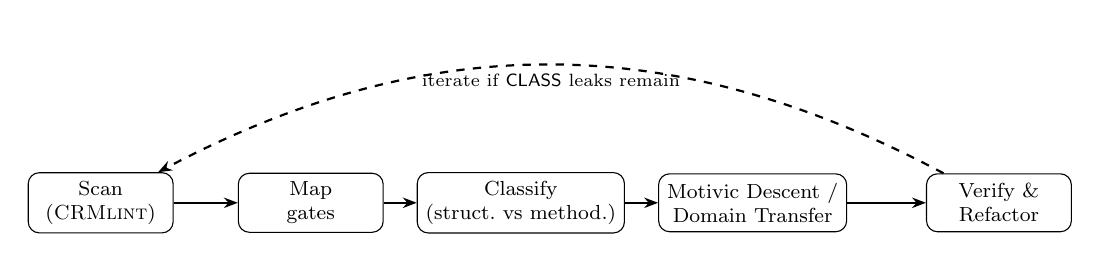
\begin{tikzpicture}[
    box/.style={draw, rounded corners, minimum width=2.0cm,
                minimum height=0.8cm, align=center, font=\footnotesize},
    arr/.style={-{Stealth[length=5pt]}, thick},
    >=Stealth,
    scale=0.92, transform shape
]
  \node[box] (scan) at (0,0) {Scan\\(\CRMlint)};
  \node[box] (map) at (2.9,0) {Map\\gates};
  \node[box] (classify) at (5.8,0) {Classify\\(struct.\ vs method.)};
  \node[box] (search) at (9.0,0) {Motivic Descent /\\Domain Transfer};
  \node[box] (verify) at (12.4,0) {Verify \&\\Refactor};

  \draw[arr] (scan) -- (map);
  \draw[arr] (map) -- (classify);
  \draw[arr] (classify) -- (search);
  \draw[arr] (search) -- (verify);
  \draw[arr, dashed] (verify) to[bend right=28] node[below,font=\scriptsize]
    {iterate if $\CLASS$ leaks remain} (scan);
\end{tikzpicture}
\caption{The upgraded scan-map-classify-search-verify loop, featuring Motivic Descent.}
\label{fig:loop}
\end{figure}

The ultimate promise of this methodology is economic. By running \CRMlint\ on a LaTeX blueprint, a formalization team can identify and mathematically excise classical parasitic dependencies, saving thousands of hours of formalization labor by ensuring the architecture is constructively optimal before the programming begins.


\subsection{The Mathematics of the LTE}\label{part:math}

This part is expository.  We restate the main theorems of the LTE
in the form proved by Scholze, Commelin, and Massot, and annotate
each step with its CRM level.  Nothing here is new mathematics.
The proofs are theirs; the CRM labels are ours.  The labels may
be useful for readers approaching the LTE from the constructive
side, or for formalization teams deciding which components to
port to Lean~4.

\subsubsection{The main theorem and its reduction}\label{sec:main-thm}

The LTE establishes the following vanishing result, which
Scholze proposed as a challenge in December 2020.

\begin{theorem}[Clausen--Scholze {\cite{scholze-lte}}]\label{thm:lte-main}
Let $0 < p' < p \leq 1$ be real numbers, let $S$ be a profinite set,
and let $V$ be a $p$-Banach space.  Let $\mathcal{M}_{p'}(S)$ denote
the space of real $p'$-measures on~$S$.  Then
\[
  \mathrm{Ext}^i_{\mathrm{Cond}(\mathrm{Ab})}(\mathcal{M}_{p'}(S),\, V) = 0
  \qquad \text{for all } i \geq 1.
\]
\end{theorem}

The Ext-groups are computed in the abelian category of condensed
abelian groups.  The theorem says: from the perspective of homological
algebra in the condensed world, real-valued measures are
``projective-like'' --- they have no higher Ext against Banach targets.

\medskip
\noindent\textbf{CRM annotation.}
The \emph{statement} of Theorem~\ref{thm:lte-main} requires:
\begin{itemize}[nosep]
\item $p$-Banach space $V$: the norm $\|\cdot\|$ on $V$ satisfies
  $\|x + y\|^p \leq \|x\|^p + \|y\|^p$.  Defining
  this norm and its completeness is $\WLPO$.
\item The condensed abelian group $\mathcal{M}_{p'}(S)$:
  defined via a filtration $\mathcal{M}_{p'}(S)_{\leq c}$, each
  level a compact Hausdorff space.  The filtration cut-off is $\LPO$.
\item Profinite $S$: a cofiltered limit of finite sets.  All $\BISH$.
\end{itemize}

\noindent The \emph{proof} reduces Theorem~\ref{thm:lte-main} to a
chain of intermediate results, each of which we now state.

\subsubsection{The proof chain: six links}\label{sec:proof-chain}

The proof proceeds by six reductions, from the main theorem down to
the key technical result (Theorem~\ref{thm:94}).  We trace the full
chain and label each link with its CRM level.

\begin{center}
\small
\begin{tabular}{clll}
\toprule
\textbf{Link} & \textbf{Result} & \textbf{Mechanism} & \textbf{CRM} \\
\midrule
6 & Theorem~\ref{thm:lte-main} (main) &
  Long exact Ext sequence from Link~5 & $\BISH$ \\
5 & Ext-vanishing for $\mathcal{L}_{r'}(S)$ &
  $T^{-1}$-bijectivity via Link~4 & $\BISH$ \\
4 & Ext-vanishing for $\overline{\mathcal{L}}_{r'}(S)$ &
  Pro-isomorphism + derived limit via Link~3 & $\BISH$ \\
3 & Theorem~\ref{thm:94} (Ext-vanishing at finite level) &
  Double complex + spectral proposition & $\LPO$ \\
2 & Column exactness (Proposition~\ref{prop:col-exact}) &
  \v{C}ech nerve + normed snake lemma & $\LPO$ \\
1 & \v{C}ech exactness (Proposition~\ref{prop:cech-exact}) &
  Contracting homotopy + profinite limit & $\BISH$/$\WKL$ \\
\bottomrule
\end{tabular}
\end{center}

\paragraph{Link 1: \v{C}ech nerve exactness ($\BISH$/$\WKL$)}

\begin{proposition}[\v{C}ech cover exactness {\cite{commelin-massot-lte}}]
\label{prop:cech-exact}
Let $\pi: X \to B$ be a surjective morphism of profinite sets,
and let $S_\bullet \to S_{-1}$, $S_{-1} := B$, be its augmented
\v{C}ech nerve.  Let $V$ be a semi-normed group.  Then the complex
\[
  0 \longrightarrow \widehat{V}(S_{-1}) \longrightarrow
  \widehat{V}(S_0) \longrightarrow
  \widehat{V}(S_1) \longrightarrow \cdots
\]
is exact.  Moreover, for every $\varepsilon > 0$ and
$f \in \ker(\widehat{V}(S_m) \to \widehat{V}(S_{m+1}))$,
there exists $g \in \widehat{V}(S_{m-1})$ with $d(g) = f$
and $\|g\| \leq (1 + \varepsilon)\|f\|$.
\end{proposition}

\noindent\textbf{Proof sketch.}
For \emph{finite} $X$ and $B$, a section $\sigma: B \to X$ of $\pi$
induces maps $S_m \to S_{m+1}$ via
$(a_0, \ldots, a_m) \mapsto (\sigma(\pi(a_0)), a_0, \ldots, a_m)$.
These provide a contracting homotopy for the complex, and the homotopy
maps are norm-nonincreasing.  For general profinite sets, write
$X = \varprojlim_i X_i$ over its discrete (finite) quotients,
pass to finite quotients $X_i \to B_i$, apply the finite case, and
take the cofiltered limit.  Surjectivity of transition maps between
compact Hausdorff spaces is preserved under cofiltered limits
(by Tychonoff).

\medskip
\noindent\textbf{CRM annotation.}
The finite case is entirely $\BISH$: the section $\sigma$ exists
because $\pi$ is surjective between finite sets, and the contracting
homotopy is an explicit combinatorial construction.  The passage to
profinite limits uses Tychonoff's theorem for compact Hausdorff spaces
(surjections of compact spaces remain surjective under cofiltered
limits).  In CRM terms, Tychonoff for Hausdorff spaces is $\WKL$
(equivalent to weak K\"onig's lemma: an infinite finitely-branching
tree has an infinite path).  The norm estimates ($\|g\| \leq
(1+\varepsilon)\|f\|$) do not introduce additional logical cost.

\paragraph{Link 2: Column exactness via normed snake lemma ($\LPO$)}

The double complex construction requires that each column is
``weakly bounded exact.''  This is established by combining
\v{C}ech exactness (Link~1) with the normed $T^{-1}$-action.

\begin{definition}[Weak bounded exactness {\cite{commelin-massot-lte}}]
\label{def:weak-exact}
A system of complexes $C_\bullet^\bullet$ is
\emph{weakly $\leq k$-exact in degrees $\leq m$ for $c \geq c_0$
with bound~$K$} if for all $c \geq c_0$, all $x \in C_{kc}^i$ with
$i \leq m$, and any $\varepsilon > 0$, there exists $y \in C_c^{i-1}$
with
\[
  \|x_{|c} - dy\| \leq K\|dx\| + \varepsilon.
\]
\end{definition}

\begin{proposition}[Column exactness {\cite{commelin-massot-lte}}]
\label{prop:col-exact}
Let $k > 1$, $c_0 > 0$ with $(k-1)c_0/N \geq d$ (the splittability
error).  Let $m$ be any natural number, and put
\[
  K = (m+2) + \frac{r+1}{r(1-r)}(m+2)^2.
\]
Then the $i$-th column in the double complex is $(k^2, K)$-weakly
bounded exact in degrees $\leq m$ for $c \geq c_0'$.
\end{proposition}

\noindent\textbf{Proof sketch.}
The key input is the ``normed dual snake lemma''
(Proposition~\ref{prop:snake} below): given two admissible systems of
complexes $M_\bullet^\bullet$ and ${M'}_\bullet^\bullet$ with a map
$f: M \to M'$, if both $M$ and $M'$ are weakly bounded exact, then
the kernel complex inherits weak bounded exactness (with controlled
loss in the constants).  The column is built from the Čech nerve of
the summation map $M^N_{c/N} \to M_c$, and the $T^{-1}$-action
introduces the norm scaling.

\medskip
\noindent\textbf{CRM annotation.}
The splittability lemma ($N$-splittability of $\mathrm{Hom}(\Lambda,
\overline{\mathcal{L}}_{r'}(S))$) is $\BISH$: it decomposes elements
of a polyhedral lattice module into $N$ pieces of roughly $1/N$-th
the norm.  The column exactness proof combines this with the $\LPO$
content of the filtration cut-offs $M_{\leq c}$.  The constant~$K$
depends on $m$ and $r$ (not on the profinite set $S$ or the normed
module $V$), so the ``universal'' part of the proof is $\BISH$ and
the $\LPO$ enters only at the interface where elements are tested
against filtration levels.

\paragraph{Link 3: The key technical result ($\LPO$)}

\begin{theorem}[Theorem 9.4 {\cite{scholze-condensed, commelin-massot-lte}}]
\label{thm:94}
Let $\mathrm{BD} = (n, f, h)$ be a Breen--Deligne package, and let
$\kappa = (\kappa_0, \kappa_1, \ldots)$ be a sequence of constants
in $\R_{\geq 0}$ that is $\mathrm{BD}$-suitable.  Fix radii
$1 > r' > r > 0$.  For any $m$ there exist $k$ and $c_0$ such that
for all profinite sets $S$ and all $r$-normed
$\Z[T^{\pm 1}]$-modules~$V$, the system of complexes
\[
  C^{\mathrm{BD}}_\kappa(\overline{\mathcal{L}}_{r'}(S))^\bullet_c
  \colon \;
  \widehat{V}(\overline{\mathcal{L}}_{r'}(S)_{\leq c})^{T^{-1}}
  \longrightarrow
  \widehat{V}(\overline{\mathcal{L}}_{r'}(S)_{\leq \kappa_1 c}^2)^{T^{-1}}
  \longrightarrow \cdots
\]
is $\leq k$-exact in degrees $\leq m$ for $c \geq c_0$.
\end{theorem}

\noindent\textbf{Proof structure.}
The proof is by induction on $m$.  The inductive step requires a
\emph{stronger} statement (Theorem~9.5$'$ in the blueprint), which
introduces a polyhedral lattice $\Lambda$ and replaces
$\overline{\mathcal{L}}_{r'}(S)$ by
$\mathrm{Hom}(\Lambda, \overline{\mathcal{L}}_{r'}(S))$.
Theorem~\ref{thm:94} is recovered by setting $\Lambda = \Z$.

The inductive step constructs a \emph{system of double complexes}:
\begin{enumerate}[nosep]
\item \textbf{Rows:} Apply the Breen--Deligne system functor to
  $\mathrm{Hom}(\Lambda^{(\bullet)}, M)$, where $\Lambda^{(\bullet)}$
  is the cosimplicial polyhedral lattice and $M$ abbreviates
  $\overline{\mathcal{L}}_{r'}(S)$.  Take the alternating face map
  complex.  Rescale norms by $m!$ for admissibility.
\item \textbf{Columns:} The column at index~$i$ is the Čech nerve
  construction of Link~2, applied with the $i$-th Breen--Deligne data.
\item \textbf{Homotopy:} The Breen--Deligne homotopy $h^N$ (the
  $N$-fold composition of the package's built-in homotopy) provides
  maps $M^{0,q+1}_{k'c} \to M^{1,q}_c$ bounded by some constant~$H$.
  The ``homotopic map'' $\delta^{0,q}_c$ factors through a deep
  restriction and has norm $\leq \varepsilon$.
\end{enumerate}

\noindent The three ingredients (row exactness by induction, column
exactness from Link~2, homotopy condition) are fed into the
\emph{spectral proposition} (Proposition~\ref{prop:spectral} below),
which yields weak bounded exactness of the first row---completing
the induction.

\medskip
\noindent\textbf{CRM annotation.}
The double complex construction (cosimplicial lattice, alternating
face map, norm rescaling) is $\BISH$: it is combinatorial algebra
over $\Z$.  The Breen--Deligne resolution itself is $\BISH$: it is a
functorial resolution of abelian groups by free modules, specified by
integer matrices.  The homotopy bound~$H$ is computed from the
Breen--Deligne data and $r, r'$---a finite computation over $\Q$,
hence $\BISH$.

The $\LPO$ enters at two points: (i) the filtration cut-offs
$\overline{\mathcal{L}}_{r'}(S)_{\leq c}$ in the system of complexes,
and (ii) the norm estimate $r^b N \leq \varepsilon$ (choosing $b$
so that $2k'(r/r')^b \leq \varepsilon$), which requires comparing
real numbers.  The choice of $N$ as a power of~2 satisfying
$k'/N \leq (r')^b$ is a single $\LPO$ decision on the ordered
reals.

\paragraph{Links 4--6: Algebraic reductions ($\BISH$)}

\noindent\textbf{Link 4: From finite level to $\overline{\mathcal{L}}_{r'}(S)$.}
Write $Q'(\overline{\mathcal{M}}_{r'}(S)) = \varinjlim_c
Q'(\overline{\mathcal{M}}_{r'}(S))_{\leq c}$ and reduce to a
pro-isomorphism statement at each finite level.  The passage to the
derived limit uses a resolution
$0 \to \bigoplus_n Q'_{\leq n} \to \bigoplus_n Q'_{\leq n} \to
Q' \to 0$
and checks that the relevant squares are bicartesian (vertical kernels
and cokernels form pro-zero systems).  This is diagram chasing in
$\mathrm{Cond}(\mathrm{Ab})$, entirely $\BISH$.

\medskip
\noindent\textbf{Link 5: From $\overline{\mathcal{L}}_{r'}(S)$
to $\mathcal{L}_{r'}(S)$.}
The short exact sequence
\[
  0 \longrightarrow \Z[T^{-1}][S] \longrightarrow
  \mathcal{L}_{r'}(S) \longrightarrow
  \overline{\mathcal{L}}_{r'}(S) \longrightarrow 0
\]
decomposes Laurent measures into negative and positive parts.
Apply $\mathrm{Ext}^*(\_, V)$: the $\Z[T^{-1}][S]$-term has
vanishing higher Ext (because $\Z[S]$ is free), and the
$\overline{\mathcal{L}}_{r'}(S)$-term vanishes by Link~4.
The five lemma gives vanishing for $\mathcal{L}_{r'}(S)$.
This is abstract homological algebra, all $\BISH$.

\medskip
\noindent\textbf{Link 6: Main theorem.}
The short exact sequence
\[
  0 \longrightarrow \mathcal{L}_{r'}(S) \xrightarrow{2T-1}
  \mathcal{L}_{r'}(S) \longrightarrow
  \mathcal{M}_{p'}(S) \longrightarrow 0
\]
(evaluation at $T = 1/2$) reduces the main theorem to the Ext-vanishing
of $\mathcal{L}_{r'}(S)$ from Link~5 via the long exact sequence.
The surjectivity of evaluation at $T = 1/2$ on pseudo-normed groups
is a norm estimate (strong exactness), which uses
Tychonoff ($\WKL$) for passage to profinite limits.  But the
long-exact-sequence argument itself is $\BISH$.


\subsubsection{The normed homological algebra toolkit}\label{sec:toolkit}

The LTE's main technical innovation is not the theorem statement
but the \emph{toolkit}: a library of normed homological algebra
results with explicit quantitative control.  These results are
general-purpose and transfer directly to other formalization targets.

\paragraph{Controlled surjectivity}

\begin{lemma}[Closure surjectivity {\cite{commelin-massot-lte}}]
\label{lem:closure-surj}
Let $G$ and $H$ be normed groups, $K \leq H$ a subgroup, and
$f: G \to H$ a $C$-surjective morphism onto $K$ (i.e., for all
$x \in K$ there exists $g$ with $f(g) = x$ and
$\|g\| \leq C\|x\|$).  If $G$ is complete, then $f$ is
$(C+\varepsilon)$-surjective onto $\overline{K}$ for every
$\varepsilon > 0$.
\end{lemma}

\noindent\textbf{Proof idea.}
Write $x \in \overline{K}$ as $x = \sum_{i \geq 0} x_i$ with
$x_i \in K$ and $\|x_i\| \leq \varepsilon_i$ for a rapidly
decreasing sequence.  Lift each $x_i$ to $g_i$ with
$\|g_i\| \leq C\|x_i\|$, and set $g = \sum g_i$.  Completeness
of $G$ guarantees convergence.  The norm estimate
$\|g\| \leq (C+\varepsilon)\|x\|$ follows from the geometric
series bound on the $\varepsilon_i$.

\medskip
\noindent\textbf{CRM annotation.}
The proof uses completeness of $G$ (to sum the Cauchy series
$\sum g_i$), which is $\WLPO$ (Cauchy convergence test).  The
lifting $x_i \mapsto g_i$ uses the $C$-surjectivity hypothesis,
which is $\BISH$ (explicit choice of lifts).  The norm comparison
$\|g_i\| \leq C\|x_i\|$ is an inequality between real numbers
($\LPO$).

\paragraph{Controlled exactness}

\begin{lemma}[Controlled exactness {\cite{commelin-massot-lte}}]
\label{lem:controlled-exact}
Let $f: M_0 \to M_1$ and $g: M_1 \to M_2$ be bounded maps between
normed groups.  Suppose $f$ is $C$-surjective onto $\ker g$, and
$g$ is $D$-surjective onto its image.  Then for every
$\varepsilon > 0$, the completion $\widehat{f}$ is
$(C+\varepsilon)$-surjective onto $\ker \widehat{g}$.
\end{lemma}

\noindent This is the mechanism by which the LTE passes from
``incomplete'' exactness (at the pre-completion level, $\BISH$) to
``completed'' exactness (at the normed-completion level, $\WLPO$).
The upgrade is Lemma~\ref{lem:closure-surj} applied to $K = \ker g$
inside $\widehat{M_1}$.

\paragraph{The normed snake lemma}

\begin{proposition}[Weak normed snake lemma {\cite{commelin-massot-lte}}]
\label{prop:snake}
Let $M_\bullet^\bullet$ and ${M'}_\bullet^\bullet$ be two admissible
systems of complexes of complete normed abelian groups, with a
norm-nonincreasing map $f: M \to M'$ satisfying
$\|x_{|c}\| \leq K'' \|f(x)\|$ for all $x \in M^i_{k''c}$,
$i \leq m+1$.  If $M$ is weakly $\leq k$-exact with bound~$K$
and $M'$ is weakly $\leq k'$-exact with bound~$K'$, then the
quotient $N = M'/M$ is weakly $\leq kk'k''$-exact in degrees
$\leq m-1$ with bound $K'(KK''+1)$.
\end{proposition}

\noindent\textbf{CRM annotation.}
The proof is a quantitative diagram chase: lift $n \in N^i$ to
$m' \in M'^i$, decompose $dm'$ using the quotient norm, apply
weak exactness of $M$ and $M'$, and track constants through.
The diagram chase is $\BISH$; the norm estimates are $\LPO$.
The bound $K'(KK''+1)$ is explicit and computable.

The \emph{dual} snake lemma (for kernels instead of cokernels)
is proved analogously, with bound $K + r_1 r_2 K K'$.
Both versions are used in the inductive step of Theorem~\ref{thm:94}:
the snake lemma produces column exactness,
and the dual snake lemma produces the kernel
complex for the $T^{-1}$-action.

\paragraph{The spectral proposition}

\begin{proposition}[Spectral proposition {\cite{commelin-massot-lte}}]
\label{prop:spectral}
Fix $m \geq 0$ and constants $k, K$.  There exist $\varepsilon > 0$
and $k_0, K_0$ (depending only on $k, K, m$) such that: if
a system of double complexes $M^{p,q}_c$ is admissible and satisfies
\begin{enumerate}[nosep,label=(\roman*)]
\item rows are weakly $\leq k$-exact in degrees $\leq m-1$ with
  bound~$K$ (for $i = 0, \ldots, m+1$),
\item columns are weakly $\leq k$-exact in degrees $\leq m$ with
  bound~$K$,
\item the normed spectral homotopy condition for $m$, some $H > 0$,
  $c_0$, and~$\varepsilon$,
\end{enumerate}
then the first row is weakly $\leq k'^2$-exact in degrees $\leq m$
with bound $2K_0 H$.
\end{proposition}

\noindent This is the engine of the induction.  The base case ($m=0$)
uses $\varepsilon = 1/(2k)$ and the homotopy condition to absorb the
$\varepsilon$-term.  The inductive step passes to the quotient complex
$N^{p,0} = M^{p,1}/\overline{M^{p,0}}$ and applies the snake lemma
(Proposition~\ref{prop:snake}) to verify the hypotheses for $m-1$.

\medskip
\noindent\textbf{CRM annotation.}
The spectral proposition is $\BISH$ in its logical content: it is a
statement about constants and admissibility conditions.  The $\LPO$
enters only when the proposition is \emph{applied} to a specific
system of double complexes built from normed groups.  This separation
is a paradigm case of the concentration thesis: the abstract machinery
is logically free, and the analytic cost is paid only at the
point of application.


\subsubsection{The Breen--Deligne resolution: pure algebra}\label{sec:BD}

The deepest algebraic ingredient in the LTE is the Breen--Deligne
resolution, which provides a functorial free resolution of any
abelian group~$A$.

\begin{theorem}[Breen--Deligne {\cite{breen-deligne}}]
For any abelian group $A$, there is a resolution, functorial in~$A$:
\[
  \cdots \longrightarrow \bigoplus_{i} \Z[A^{r_{ij}}]
  \longrightarrow \cdots
  \longrightarrow \Z[A^3] \oplus \Z[A^2]
  \longrightarrow \Z[A^2]
  \longrightarrow \Z[A]
  \longrightarrow A \longrightarrow 0.
\]
The functorial maps $\Z[A^m] \to \Z[A^n]$ are specified by
integer matrices (``basic universal maps'': $n \times m$ matrices
over $\Z$), composed via matrix multiplication.
\end{theorem}

\noindent\textbf{CRM annotation.}
The entire Breen--Deligne resolution---its existence, functoriality,
and the universal maps---is $\BISH$.  The universal maps are
$\Z$-linear combinations of basic universal maps specified by
integer matrices; their composition is matrix multiplication; the
homotopy $h$ packaged with the resolution is a universal map bounded
by an integer~$N$.  No real analysis, no completeness, no decidability
of real arithmetic appears anywhere.  Just as Scholze's motivic
geometric Satake achieves $\BISH$ by replacing analytic intersection
cohomology with algebraic MV~cycles (\S\ref{sec:audit}), the
Breen--Deligne resolution achieves $\BISH$ by replacing analytic
bounds with integer matrices.

This is the algebraic skeleton of the LTE in its purest form.
The LTE formalizes it in Lean~3 as
\texttt{breen\_deligne.basic\_universal\_map} (integer matrices),
\texttt{breen\_deligne.universal\_map} (formal $\Z$-linear
combinations), and \texttt{breen\_deligne.package} (the triple
$(n, f, h)$).

\subsubsection{What transfers: reusable components}\label{sec:reusable}

The LTE's mathematical infrastructure divides into three categories
by reusability.

\paragraph{Category A: Directly reusable ($\BISH$)}

These components depend on no analytic input and can be ported to
Lean~4 as standalone libraries.

\begin{enumerate}[nosep]
\item \textbf{Breen--Deligne package.}  Integer matrices, universal
  maps, the package triple $(n, f, h)$, homotopy composition
  $h^N$, suitability conditions on $\kappa$.  All finitary
  algebra over $\Z$.

\item \textbf{Polyhedral lattices.}  Finite free abelian groups with
  generating norms.  The key combinatorial lemma:
  $N$-splittability of $\mathrm{Hom}(\Lambda,
  \overline{\mathcal{L}}_{r'}(S))$ with explicit error term~$d$.

\item \textbf{Cosimplicial polyhedral lattices.}
  $\Lambda' = \Lambda^N$ with the $\ell^1$-norm; the cosimplicial
  object $\Lambda^{(\bullet)}$; the Čech nerve isomorphisms
  $\mathrm{Hom}(\Lambda'^{(m)}, M)_{\leq c} \cong
  \mathrm{Hom}(\Lambda', M)_{\leq c}^{m /
  \mathrm{Hom}(\Lambda, M)_{\leq c}}$.

\item \textbf{Abstract diagram chasing.}  The pro-isomorphism
  argument (Link~4), the five-lemma reduction (Link~5), the
  short-exact-sequence reduction (Link~6).
\end{enumerate}

\paragraph{Category B: Reusable with $\LPO$ interface ($\LPO$)}

These components are algebraic in structure but require norm
comparisons at the interface.

\begin{enumerate}[nosep]
\item \textbf{Systems of complexes.}  Functors
  $(\R_{\geq 0})^{\mathrm{op}} \to \mathrm{Ch}(\mathrm{SemiNormGrp})$.
  The restriction maps $\mathrm{res}_{c',c}$ require
  $c' \geq c$ ($\LPO$).  The definitions of $\leq k$-exactness,
  weak $\leq k$-exactness, and admissibility are $\BISH$
  conditions on the norms.

\item \textbf{The spectral proposition.}
  The statement and proof of Proposition~\ref{prop:spectral}
  are $\BISH$ as abstract algebra.  The $\LPO$ enters only at
  instantiation.

\item \textbf{The normed snake lemma (both versions).}
  The diagram chase is $\BISH$; the norm bounds use
  $\LPO$.
\end{enumerate}

\paragraph{Category C: Analytic core ($\WLPO$/$\LPO$)}

These components are irreducibly analytic.

\begin{enumerate}[nosep]
\item \textbf{Normed completions $\widehat{V}(\cdot)$.}
  The completion functor on semi-normed groups.  Cauchy
  convergence is $\WLPO$; the norm on the completion is $\LPO$.

\item \textbf{The $T^{-1}$-action on $\overline{\mathcal{L}}_{r'}(S)$.}
  The shift $T^{-1} \cdot (\sum a_n T^n) = (\sum a_{n+1} T^n)$
  scales the norm by $r'$: the filtration level changes from
  $\leq c$ to $\leq c/r'$.  This scaling requires norm
  comparison ($\LPO$).

\item \textbf{The homotopy norm estimate.}
  The key bound $r^b N \leq \varepsilon$ (choosing $b$ so that
  $2k'(r/r')^b \leq \varepsilon$) requires decidable ordering
  on $\R$ ($\LPO$).  This is the deepest analytic content in
  the entire proof: a single real-number comparison that
  controls the convergence of the induction.
\end{enumerate}

\subsubsection{Lean~4 formalization targets}\label{sec:lean4}

The LTE was formalized in Lean~3 (community \texttt{mathlib} fork).
A Lean~4 port faces the standard Lean~3 $\to$ Lean~4 translation
burden, but the \emph{mathematical} targets are well-defined.
We identify the most valuable targets from the CRM perspective:
components where the $\BISH$/$\LPO$ separation is sharpest and
the reuse potential is highest.

\paragraph{Target 1: Breen--Deligne package (pure $\BISH$)}

\begin{verbatim}
-- Basic universal maps: integer matrices
structure BasicUniversalMap (m n : Nat) where
  matrix : Matrix (Fin n) (Fin m) Int

-- Universal maps: formal Z-linear combinations
structure UniversalMap (m n : Nat) where
  terms : List (Int x BasicUniversalMap m n)

-- Composition via matrix multiplication
def UniversalMap.comp (f : UniversalMap m n)
    (g : UniversalMap l m) : UniversalMap l n := ...

-- BD package: exponents, differentials, homotopy
structure BDPackage where
  n : Nat -> Nat                  -- exponents
  f : (i : Nat) -> UniversalMap (n (i+1)) (n i)
  h : (i : Nat) -> UniversalMap (n (i+1)) (n i)
  chain_complex : forall i, (f i).comp (f (i+1)) = 0
  homotopy_rel : forall i, ...   -- h witnesses null-homotopy
\end{verbatim}

This is finite combinatorics over $\Z$.  No axioms beyond
\texttt{propext} and \texttt{Quot.sound}.  The key theorem to
formalize: given a BD package and a suitable sequence $\kappa$,
the $N$-fold homotopy $h^N$ exists and is bounded by an explicit
integer.

\paragraph{Target 2: Systems of complexes ($\BISH$ definitions, $\LPO$ at interface)}

\begin{verbatim}
-- System of complexes: parametrized by NNReal
structure SystemOfComplexes where
  C : NNReal -> ChainComplex SemiNormedGroup
  res : forall c' c, c' >= c -> C c' --> C c
  res_comp : forall c'' c' c (h1 : c'' >= c')
    (h2 : c' >= c), res c'' c (le_trans h2 h1) =
    (res c' c h2).comp (res c'' c' h1)

-- Weak bounded exactness
def SystemOfComplexes.IsWeakBoundedExact
    (S : SystemOfComplexes) (k K : Real) (m : Nat)
    (c0 : NNReal) : Prop :=
  forall c >= c0, forall i <= m,
    forall x in (S.C (k * c)).obj i,
    forall eps > 0, exists y in (S.C c).obj (i-1),
      norm (res x - d y) <= K * norm (d x) + eps
\end{verbatim}

The definition is $\BISH$.  The $\LPO$ enters at the inequality
$c' \geq c$ (comparison of real numbers) and the norm estimate.

\paragraph{Target 3: Controlled surjectivity lemma ($\WLPO$)}

\begin{verbatim}
-- Key lemma: C-surjectivity extends to closures
theorem controlled_closure_of_complete
    {G H : NormedAddCommGroup} [CompleteSpace G]
    {K : AddSubgroup H} {f : G ->+ H} {C : Real}
    (hf : forall x in K,
      exists g, f g = x && norm g <= C * norm x)
    (eps : Real) (heps : 0 < eps) :
    forall x in K.topologicalClosure,
      exists g, f g = x
        && norm g <= (C + eps) * norm x := by
  -- Proof: geometric series in complete G
  ...
\end{verbatim}

This requires \texttt{CompleteSpace G} ($\WLPO$: Cauchy sequences
converge) and the norm bound ($\LPO$: $\|g\| \leq C\|x\|$).
The Lean~4 proof would use \texttt{Metric.cauchySeq\_of\_le\_geometric}
from Mathlib.

\paragraph{Target 4: Normed snake lemma ($\BISH$ chase, $\LPO$ bounds)}

The most technically demanding target.  The Lean~3 proof
(\texttt{weak\_normed\_snake} and \texttt{weak\_normed\_snake\_dual})
runs approximately 200 lines.  A Lean~4 port would:
\begin{itemize}[nosep]
\item Define admissible systems of complexes over Mathlib's
  \texttt{SemiNormedGroup}.
\item Implement the quantitative diagram chase with explicit
  $\varepsilon$-management.
\item Prove the bound $K'(KK''+1)$ for quotients and
  $K + r_1 r_2 K K'$ for kernels.
\end{itemize}

The entire chase is $\BISH$ (diagram manipulation in an abelian
category with explicit lifts).  The $\LPO$ enters only at the
final norm inequality.

\paragraph{CRM summary of formalization targets}

\begin{center}
\begin{tabular}{llcl}
\toprule
\textbf{Target} & \textbf{Component} & \textbf{CRM} & \textbf{Lean~4 difficulty} \\
\midrule
1 & Breen--Deligne package  & $\BISH$ & Low (finite algebra over $\Z$) \\
2 & Systems of complexes    & $\BISH$/$\LPO$ & Medium (parametrized complexes) \\
3 & Controlled surjectivity & $\WLPO$ & Low (standard Cauchy argument) \\
4 & Normed snake lemma      & $\BISH$/$\LPO$ & High (200-line diagram chase) \\
\bottomrule
\end{tabular}
\end{center}

Targets~1 and~3 are low-hanging fruit: they are self-contained,
well-typed, and already have Lean~3 implementations to translate.
Target~2 requires design decisions about how to interface
with Mathlib's \texttt{CategoryTheory.ChainComplex}.
Target~4 is the highest-value formalization: the normed snake
lemma is the engine of the induction, and a clean Lean~4
version would serve as infrastructure for any future normed
homological algebra project.

\medskip
\noindent\textbf{Acknowledgments for this appendix.}
The LTE blueprint files used in this analysis were authored by Johan Commelin
and Patrick Massot~\cite{commelin-massot-lte}. The mathematical content follows
the proofs in~\cite{scholze-condensed} as formalized in~\cite{commelin-massot-lte}.


%======================================================================
\begin{thebibliography}{99}

\bibitem{scholze-berkovich} P.\ Scholze, Berkovich motives, arXiv:2412.03382, 2024 (revised January 2026).

\bibitem{scholze-motivic-geometrization} P.\ Scholze, Geometrization of the local Langlands correspondence, motivically, arXiv:2501.07944, January 2026.

\bibitem{fargues-scholze21} L.\ Fargues and P.\ Scholze, Geometrization of the local Langlands correspondence, arXiv:2102.13459, to appear in Ast\'erisque, 2021.

\bibitem{lee-p98} P.\ C.-K.\ Lee, The motivic CRM architecture: why the six domains of mathematics have different logical signatures, and how motives explain the pattern (Paper~98), Zenodo, 2026. DOI: \href{https://doi.org/10.5281/zenodo.18902037}{10.5281/zenodo.18902037}.

\bibitem{richarz-scholbach} T.\ Richarz and J.\ Scholbach, The motivic Satake equivalence, \emph{Math.\ Ann.} 380 (2021), 1595--1653.

\bibitem{cass-vdh-scholbach} R.\ Cass, T.\ van den Hove, and J.\ Scholbach, The geometric Satake equivalence for integral motives, preprint.

\bibitem{bishop67} E.\ Bishop, \emph{Foundations of Constructive Analysis}, McGraw-Hill, 1967.

\bibitem{bridges-richman87} D.\ Bridges and F.\ Richman, \emph{Varieties of Constructive Mathematics}, LMS Lecture Notes 97, Cambridge, 1987.

\bibitem{ishihara06} H.\ Ishihara, Reverse mathematics in Bishop's constructive mathematics, \emph{Phil.\ Sci.\ Cahier Sp\'ecial} 6 (2006), 43--59.

\bibitem{wiles95} A.\ Wiles, Modular elliptic curves and Fermat's Last Theorem, \emph{Ann.\ of Math.} 141 (1995), 443--551.

\bibitem{taylor-wiles95} R.\ Taylor and A.\ Wiles, Ring-theoretic properties of certain Hecke algebras, \emph{Ann.\ of Math.} 141 (1995), 553--572.

\bibitem{lafforgue02} L.\ Lafforgue, Chtoucas de Drinfeld et correspondance de Langlands, \emph{Invent.\ Math.} 147 (2002), 1--241.

\bibitem{arthur05} J.\ Arthur, An introduction to the trace formula, in: \emph{Harmonic Analysis, the Trace Formula, and Shimura Varieties}, Clay Math.\ Proc.\ 4, AMS, 2005, 1--263.

\bibitem{hochster69} M.\ Hochster, Prime ideal structure in commutative rings, \emph{Trans.\ Amer.\ Math.\ Soc.} 142 (1969), 43--60.

\bibitem{lee-p76} P.\ C.-K.\ Lee, CRMlint: automated logical cost analysis of mathematical proof (Paper~76), Zenodo, 2026. DOI: \href{https://doi.org/10.5281/zenodo.18779362}{10.5281/zenodo.18779362}.

\bibitem{lee-p99} P.\ C.-K.\ Lee, The Hecke theta series squeeze: resolving the dihedral base case of modularity via Mumford's algebraic theta functions (Paper~99), Zenodo, 2026.

\bibitem{lee-p100} P.\ C.-K.\ Lee, The Kuga--Satake bifurcation: absolute Hodge classes on K3 surfaces via Shioda--Inose structure (Paper~100), Zenodo, 2026.

\bibitem{crmlint-scanner} P.\ C.-K.\ Lee, CRMlint scanner output and classification for Berkovich motives and motivic geometrization, supplementary appendix to Paper~101, 2026.

\bibitem{lee-format} P.\ C.-K.\ Lee, Paper format guide for the constructive reverse mathematics series, Zenodo, 2026. DOI: \href{https://doi.org/10.5281/zenodo.18765700}{10.5281/zenodo.18765700}.

\bibitem{buzzard-perfectoid} K.\ Buzzard, J.\ Commelin, and P.\ Massot, Formalising perfectoid spaces, in: \emph{Proceedings of the 9th ACM SIGPLAN International Conference on Certified Programs and Proofs}, 2020, 299--312.

\bibitem{scholze-condensed} P.\ Scholze, Lectures on analytic geometry, lecture notes, 2019.

\bibitem{scholze-lte} P.\ Scholze, Liquid tensor experiment, 2020. Available at \url{https://xenaproject.wordpress.com/2020/12/05/}.

\bibitem{commelin-massot-lte} J.\ Commelin and P.\ Massot, Liquid tensor experiment: formal verification in Lean~3, 2022. Repository: \url{https://github.com/leanprover-community/liquid}.

\bibitem{clausen-scholze22} D.\ Clausen and P.\ Scholze, \emph{Condensed Mathematics and Complex Geometry}, 2022.

\bibitem{lee-p5} P.\ C.-K.\ Lee, General relativity is BISH + LPO: the logical cost of the equivalence principle (Paper~5), CRM Series, 2024. DOI: \href{https://doi.org/10.5281/zenodo.18765700}{10.5281/zenodo.18765700}.

\bibitem{lee-p72} P.\ C.-K.\ Lee, The DPT characterisation theorem (Paper~72), CRM Series, 2025.

\bibitem{lee-p73} P.\ C.-K.\ Lee, Axiom~1 is irreversible (Paper~73), CRM Series, 2025.

\bibitem{lee-p74} P.\ C.-K.\ Lee, Axiom~2 is irreversible (Paper~74), CRM Series, 2025.

\bibitem{lee-p77} P.\ C.-K.\ Lee, Explicit Hodge decompositions for $E^4$ (Paper~77), CRM Series, 2026. DOI: \href{https://doi.org/10.5281/zenodo.18777596}{10.5281/zenodo.18777596}.

\bibitem{lee-p78} P.\ C.-K.\ Lee, The local Langlands correspondence for $\mathrm{GL}_2(\mathbb{Q}_2)$ is constructively decidable (Paper~78), CRM Series, 2026. DOI: \href{https://doi.org/10.5281/zenodo.18789008}{10.5281/zenodo.18789008}.

\bibitem{lee-p90} P.\ C.-K.\ Lee, The squeeze is a microscope: automated constructivization from CRMLint to the Hodge horizon (Paper~90), CRM Series, 2026. DOI: \href{https://doi.org/10.5281/zenodo.18809911}{10.5281/zenodo.18809911}.

\bibitem{lee-p95} P.\ C.-K.\ Lee, The BSD squeeze: CRMLint decomposition of the Gross--Zagier--Kolyvagin proof (Paper~95), CRM Series, 2026. DOI: \href{https://doi.org/10.5281/zenodo.18821019}{10.5281/zenodo.18821019}.

\bibitem{lee-p96} P.\ C.-K.\ Lee, The root number bifurcation: CRM cost of BSD detection controlled by the functional equation (Paper~96), CRM Series, 2026. DOI: \href{https://doi.org/10.5281/zenodo.18869924}{10.5281/zenodo.18869924}.

\bibitem{mathlib4} The Mathlib Community, \emph{Mathlib4: Mathematics in Lean~4}, \url{https://github.com/leanprover-community/mathlib4}, 2024--2026.

\bibitem{simpson09} S.\ G.\ Simpson, \emph{Subsystems of Second Order Arithmetic}, 2nd ed., Cambridge University Press, 2009.

\bibitem{breen-deligne} L.\ Breen, Extensions du groupe additif, \emph{Inst.\ Hautes \'Etudes Sci.\ Publ.\ Math.}~48 (1978), 39--125.

\bibitem{tychonoff30} A.\ N.\ Tychonoff, \"Uber die topologische Erweiterung von R\"aumen, \emph{Math.\ Ann.}~102 (1930), 544--561.

\end{thebibliography}

\end{document}
